%%%%%%%%%%%%%%%%%%%%%%%%%%%%%%%%%%%%%%%%%%%%%%%%%%%%%%%%%%%%%%%%%%%%%
%
% Complete documentation on the extended LaTeX markup used for Insight
% documentation is available in ``Documenting Insight'', that is part
% of the standard documentation for Insight.  It may be found online
% at:
%
%                    http://www.itk.org
%
%%%%%%%%%%%%%%%%%%%%%%%%%%%%%%%%%%%%%%%%%%%%%%%%%%%%%%%%%%%%%%%%%%%%%

\documentclass{InsightSoftwareGuide}


\usepackage[dvips]{graphicx}
\usepackage{times,lscape,url}
%\usepackage{mdwtab}


%%% \usepackage[latin1]{inputenc}
%%% \selectlanguage{french}
% Configuration pour les accents francais pour l'OTB
\usepackage[latin1]{inputenc}
%\usepackage[french]{babel}
\usepackage{tikz}

\usepackage{color}

\definecolor{listcomment}{rgb}{0.0,0.5,0.0}
\definecolor{listkeyword}{rgb}{0.0,0.0,0.5}
\definecolor{listnumbers}{gray}{0.65}
\definecolor{listlightgray}{gray}{0.955}
\definecolor{listwhite}{gray}{1.0}

\usepackage{minted}
\newminted{cpp}{fontsize=\small}
\newminted{cmake}{fontsize=\small}
\newminted{bat}{fontsize=\small}

\usepackage{mdframed}
\BeforeBeginEnvironment{cppcode}{\begin{mdframed}[leftline=false,rightline=false,backgroundcolor=listlightgray]}
\AfterEndEnvironment{cppcode}{\end{mdframed}}

\newif\ifitkFullVersion
\itkFullVersiontrue
%\itkFullVersionfalse

\newif\ifitkPrintedVersion
\itkPrintedVersiontrue
%\itkPrintedVersionfalse

\usepackage{multicol}

%%%%%%%%%%%%%%%%%%%%%%%%%%%%%%%%%%%%%%%%%%%%%%%%%%%%%%%%%%%%%%%%%%
%
%  hyperref should be the last package to be loaded.
%
%%%%%%%%%%%%%%%%%%%%%%%%%%%%%%%%%%%%%%%%%%%%%%%%%%%%%%%%%%%%%%%%%%
\ifitkPrintedVersion
\usepackage[dvips,
pdftitle={OTB Software Guide},
pdfauthor={CNES},
pdfsubject={Remote Sensing, Orfeo, Pleiades, Cosmo Skymed},
pdfkeywords={Image processing, Remote sensing, Guide},
pdfpagemode={UseOutlines},
bookmarks,bookmarksopen,
pdfstartview={FitH},
backref,
colorlinks,linkcolor={black},citecolor={black},urlcolor={black},
]{hyperref}
\else
\usepackage[dvips,
pdftitle={OTB Software Guide},
pdfauthor={CNES},
pdfsubject={Remote Sensing, Orfeo, Pleiades, Cosmo Skymed},
pdfkeywords={Image processing, Remote sensing, Guide},
pdfpagemode={UseOutlines},
bookmarks,bookmarksopen,
pdfstartview={FitH},
backref,
colorlinks,linkcolor={blue},citecolor={blue},urlcolor={blue},
]{hyperref}
\fi

\usepackage{amsmath,amssymb,amsfonts}
\usepackage{bbm}
%%%%%%%%%%%%%%%%%%%%%%%%%%%%%%%%%%%%%%%%%%%%%%%%%%%%%%%%%%%%%%%%%%%
%
%
%   Load configuration parameters prepared by CMake
%
%
%%%%%%%%%%%%%%%%%%%%%%%%%%%%%%%%%%%%%%%%%%%%%%%%%%%%%%%%%%%%%%%%%%%

\input{SoftwareGuideConfiguration.tex}

\def\logoCNES{CNES_nom.eps}

\newtheorem{algo}{Algorithm}
\newtheorem{defin}{Definition}
%%%%%%%%%%%%%%%%%%%%%%%%%%%%%%%%%%%%%%%%%%%%%%%%%%%%%%%%%%%%%%%%%%%
%
%
%           The Insight Toolkit Software Guide
%
%
%%%%%%%%%%%%%%%%%%%%%%%%%%%%%%%%%%%%%%%%%%%%%%%%%%%%%%%%%%%%%%%%%%%

\title{The ORFEO Tool Box Software Guide\\ Updated
  for OTB-\otbversion}

\author{OTB Development Team}

\authoraddress{
  \url{http://www.orfeo-toolbox.org}\\
  e-mail: \email{otb@cnes.fr}
}

\date{\today}


% actually write the .idx file
\makeindex

\setcounter{tocdepth}{3}



%%%%%%%%%%%%%%%%%%%%%%%%%%%%%%%%%%%%%%%%%%%%%%%%%%%%%%%%%%%%%%%%%%%
%
%           Begin Document
%
%%%%%%%%%%%%%%%%%%%%%%%%%%%%%%%%%%%%%%%%%%%%%%%%%%%%%%%%%%%%%%%%%%%

\begin{document}

\ifitkPrintedVersion
%% \input{PrintedPreamble.tex}
\fi

\maketitle

\frontmatter

\hyperbaseurl{http://www.orfeo-toolbox.org}


%%%%%%%%%%%%%%%%%%%%%%%%%%%%%%%%%%%%%%%%%%
%
%  Page with OTB logo
%
%%%%%%%%%%%%%%%%%%%%%%%%%%%%%%%%%%%%%%%%%%
\cleardoublepage

\begin{minipage}[t][10cm][b]{\textwidth}
\center
\includegraphics[width=0.5\textwidth]{logoVectoriel.eps}
\large
\begin{center}
\emph{The ORFEO Toolbox is not a black box.}\\
\end{center}
\hspace{8cm} Ch.D.
\normalsize
\end{minipage}



%%%%%%%%%%%%%%%%%%%%%%%%%%%%%%%%%%%%%%%%%%%%%%
%
% remove headings from the following material
\pagestyle{plain}
%
%%%%%%%%%%%%%%%%%%%%%%%%%%%%%%%%%%%%%%%%%%%%%%



%%\ifitkPrintedVersion
%% \input{Cover.tex}
%%\fi




%%%%%%%%%%%%%%%%%%%%%%%%%%%%%%%%%%%%%%%%%%%%%%%%%%%%%%%%%
%
% Insert Table of Contents; List of Figures and Tables
%
%%%%%%%%%%%%%%%%%%%%%%%%%%%%%%%%%%%%%%%%%%%%%%%%%%%%%%%%%


%%%%%%%%%%%%%%%%%%%%%%%%%%%%%%%%%%%%%%%%%%%%%%
%
% enable headings from the following material
\pagestyle{normal}
%
%%%%%%%%%%%%%%%%%%%%%%%%%%%%%%%%%%%%%%%%%%%%%%
\small
\tableofcontents
\listoffigures
\listoftables
\normalsize




%%%%%%%%%%%%%%%%%%%%%%%%%%%%%%%%%%%%%%%%%
%
% Begin technical content
%
%%%%%%%%%%%%%%%%%%%%%%%%%%%%%%%%%%%%%%%%%

\mainmatter

\part{User's guide}\label{part:userguide}

\chapter{Data Representation}
\label{sec:DataRepresentation}

\section{Image}
\label{sec:ImageSection}

The \doxygen{otb}{Image} class follows the spirit of
\href{http://www.boost.org/more/generic_programming.html}{Generic
Programming}, where types are separated from the algorithmic behavior
of the class.  OTB supports images with any pixel type and any spatial
dimension.

\subsection{Creating an Image}\label{sec:CreatingAnImageSection}

\input{Image1.tex}

In practice it is rare to allocate and initialize an image directly.
Images are typically read from a source, such a file or data acquisition
hardware. The following example illustrates how an image can be read from
a file.




\subsection{Reading an Image from a File}
\label{sec:ReadingImageFromFile}

\input{Image2.tex}





\subsection{Accessing Pixel Data}
\label{sec:AccessingImagePixelData}

\input{Image3.tex}




\subsection{Defining Origin and Spacing}
\label{sec:DefiningImageOriginAndSpacing}

\input{Image4.tex}

\subsection{Accessing Image Metadata}
\label{sec:AccessingImageMetadata}
\input{MetadataExample}

\subsection{Vector Images}
\label{sec:DefiningVectorImages}

\input{VectorImage.tex}


\subsection{Importing Image Data from a Buffer}
\label{sec:ImportingImageDataFromABuffer}
\input{Image5.tex}

\subsection{Image Lists}
\label{sec:ImageLists}
\input{ImageListExample.tex}



2;rgb:0000/0000/0000\chapter{Reading and Writing Images}
\label{sec:IO}

This chapter describes the toolkit architecture supporting reading and
writing of images to files. OTB does not enforce any particular file
format, instead, it provides a structure inherited from ITK,
supporting a variety of formats that can be easily extended by the
user as new formats become available.

We begin the chapter with some simple examples of file I/O.

\section{Basic Example}
\label{sec:ImagReadWrite}
\input{ImageReadWrite.tex}

To better understand the IO architecture, please refer to Figures
\ref{fig:ImageIOCollaborationDiagram},
\ref{fig:ImageIOFactoriesUseCases}, and
\ref{fig:ImageIOFactoriesClassDiagram}.

\begin{figure}
\center
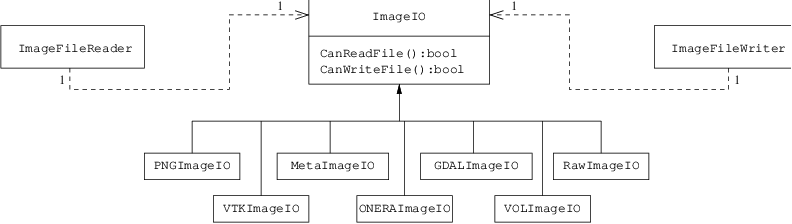
\includegraphics[width=\textwidth]{ImageIOCollaborationDiagram.eps}
\itkcaption[Collaboration diagram of the ImageIO classes]{Collaboration diagram
of the ImageIO classes.} \label{fig:ImageIOCollaborationDiagram}
\end{figure}

\begin{figure}
\center
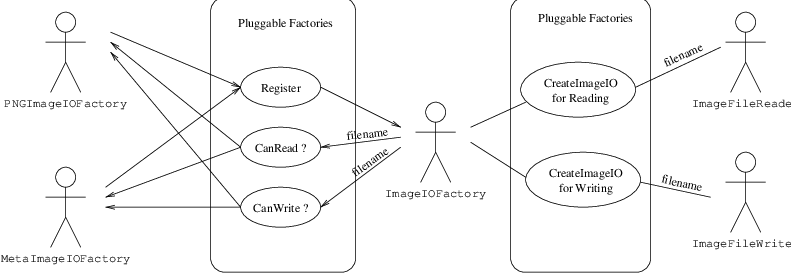
\includegraphics[width=\textwidth]{ImageIOFactoriesUseCases.eps}
\itkcaption[Use cases of ImageIO factories] {Use cases of ImageIO factories.}
\label{fig:ImageIOFactoriesUseCases}
\end{figure}

\begin{figure}
\center
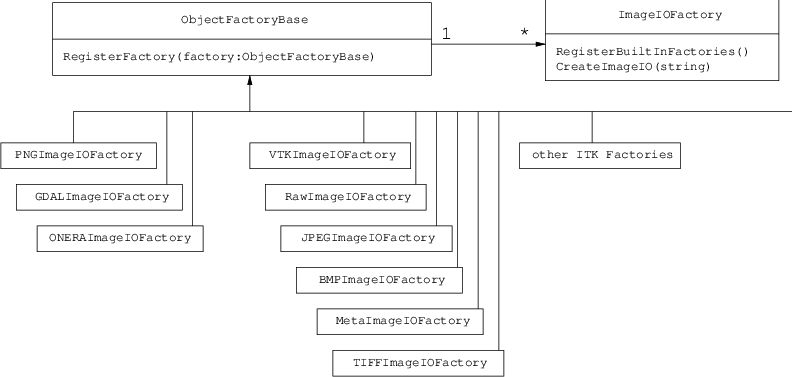
\includegraphics[width=\textwidth]{ImageIOFactoriesClassDiagram.eps}
\itkcaption[Class diagram of ImageIO factories] {Class diagram of the ImageIO
factories.}
\label{fig:ImageIOFactoriesClassDiagram}
\end{figure}


The following section describes the internals of the IO architecture provided
in the toolbox.

\section{Reading, Casting and Writing Images}
\label{sec:ImagReadCastWrite}
\input{ImageReadCastWrite.tex}

\section{Extracting Regions}
\label{sec:ImagReadRegionOfInterestWrite}
\input{ImageReadRegionOfInterestWrite.tex}


\section{Reading and Writing Vector Images}
\index{Image!Multispectral}
\label{sec:VectorImagReadWrite}

Images whose pixel type is a Vector, a CovariantVector, an Array, or a Complex
are quite common in image processing. One of the uses of these tye of
images is the processing of SLC SAR images, which are complex.


\subsection{Reading and Writing Complex Images}
\label{sec:ComplexImagReadWrite}
\input{ComplexImageReadWrite.tex}

\section{Reading and Writing Multiband Images}
\label{sec:MultibandImagReadWrite}
\input{MultibandImageReadWrite.tex}

\subsection{Extracting ROIs}
\label{sec:ExtractROI}
\input{ExtractROI.tex}

\section{Reading Image Series}
\label{sec:ReadingImageSeries}
\input{ImageSeriesIOExample}


\chapter{Reading and Writing Auxiliary Data}
\index{Auxiliary data}
\label{sec:ReadingAuxData}

As we have seen in the previous chapter, OTB has a great capability to
read and process images. However, images are not the only type of data
we will need to manipulate. Images are characterized by a regular
sampling grid. For some data, such as Digital Elevation Models (DEM)
or Lidar, this is too restrictive and we need other representations.

Vector data are also used to represent cartographic objects,
segmentation results, etc: basically, everything which can be seen as
points, lines or polygons. OTB provides functionnalities for accessing
this kind of data.

\section{Reading DEM Files}
\index{Digital elevation model}
\label{sec:ReadDEM}
\input{DEMToImageGenerator.tex}

\section{Elevation management with OTB}
\ifitkFullVersion
\label{sec:DEMHandler}
\fi
\input{DEMHandlerExample.tex}

More examples about representing DEM are presented in section~\ref{sec:ViewingAltitudeImages}.

\section{Reading and Writing Shapefiles and KML}
\index{Auxiliary data!vector data}
\index{Auxiliary data!shapefile}
\index{Auxiliary data!KML}
\label{sec:ReadVectorData}
\input{VectorDataIOExample.tex}


\chapter{Basic Filtering}


This chapter introduces the most commonly used filters found in OTB.
Most of these filters are intended to process images. They will accept one or
more images as input and will produce one or more images as output. OTB is
based ITK's data pipeline architecture in which the output of one filter is
passed as input to another filter. (See Section
\ref{sec:DataProcessingPipeline} on page \pageref{sec:DataProcessingPipeline}
for more information.)


\section{Thresholding}
\ifitkFullVersion
\label{sec:ThresholdingFiltering}
\fi

The thresholding operation is used to change or identify pixel values based
on specifying one or more values (called the \emph{threshold} value). The
following sections describe how to perform thresholding operations using
OTB.

\subsection{Threshold to Point Set}
\label{sec:ThresholdImageToPointSetFilter}

\ifitkFullVersion
\input{ThresholdToPointSetExample.tex}
\fi



\section{Mathematical operations on images}
OTB and ITK provide a lot of filters allowing to perform basic operations on image layers (thresholding, ratio, layers combinations...).
It allows to create a processing chain defining at each step operations and to combine them in the data pipeline.
But the library offers also the possibility to perform more generic complex mathematical operation on images in a single filter: the
\doxygen{otb}{BandMathImageFilter} and more recently the \doxygen{otb}{BandMathImageFilterX}.

\subsection{BandMath filter}
\label{sec:BandMathImageFilter}

\ifitkFullVersion
\input{BandMathFilterExample.tex}
\fi

\subsection{BandMathX filter}
\label{sec:BandMathImageFilterX}
A new version of the BandMath filter is now available; among the new functionalities, variables representing multi-band pixels were introduced, as well as variables representing neighborhoods of pixels. The class name is \doxygen{otb}{BandMathImageFilterX}.

\ifitkFullVersion
\input{BandMathXImageFilterExample.tex}
\fi


\subsection{Ratio of Means Detector}
\input{TouziEdgeDetectorExample}


\subsubsection{Mean Shift filtering and clustering}
\label{sec:MeanShift}

\ifitkFullVersion
\input{MeanShiftSegmentationFilterExample.tex}
\fi



\subsection{Edge Preserving Speckle Reduction Filters}
\label{sec:SpeckleFilters}
\ifitkFullVersion
\input{LeeImageFilter.tex}
\input{FrostImageFilter.tex}
\fi



\subsection{Edge preserving Markov Random Field}

The Markov Random Field framework for OTB is more detailed in \ref{sec:MarkovRandomFieldOTB} (p. \pageref{sec:MarkovRandomFieldOTB}).

\index{Markov!Filtering}
\index{Markov!Restoration}
\ifitkFullVersion
\input{MarkovRestorationExample.tex}
\fi






\chapter{Disparity Map Estimation}
\label{sec:DisparityMapEstimation}

This chapter introduces the tools available in OTB for the estimation
of geometric disparities between images.


\section{Disparity Maps}
\ifitkFullVersion
\label{sec:DisparityMaps}
\fi

The problem we want to deal with is the one of the
automatic disparity map estimation of images acquired with different sensors. By different
sensors, we mean sensors which produce images with different
radiometric properties, that is, sensors which measure different
physical magnitudes: optical sensors operating in different spectral
bands, radar and optical sensors, etc.\\

For this kind of image pairs, the classical approach of fine
correlation \cite{correl1,correl2}, can not always be used to
provide the required accuracy, since this similarity measure (the correlation
coefficient) can only measure similarities up to an affine
transformation of the radiometries.\\

There are two main questions which can be asked about what we want to
do:
\begin{enumerate}
\item Can we define what the similarity is between, for instance, a radar
and an optical image?
\item What does {\em fine registration} mean in the case where the
geometric distortions are so big and the source of information can be
located in different places (for instance, the same edge can be
produced by the edge of the roof of a building in an optical image and
by the wall-ground bounce in a radar image)?
\end{enumerate}

We can answer by saying that the images of the same object obtained by different
sensors are two different representations of the same reality. For the
same spatial location, we have two different measures. Both information
come from the same source and thus they have a lot of common
information. This relationship may not be perfect, but it can be
evaluated in a relative way: different geometrical distortions are
compared and the one leading to the strongest link between the two
measures is kept.\\

%% proposed by Ventura et al. \cite{ventura}. They even applied it to the
%% problem of image to map registration. The approach was also finding HP
%% by matching extracted features.\\


%% Dai and Khorram \cite{xiaolong} use a feature based approach: they
%% extract closed edges which are characterized using invariant
%% moments. Then, the extracted areas are matched using their
%% characterization. Finally, the centers of gravity of each area are
%% used as HP for the estimation of an affine transformation. They apply
%% the approach to Landsat images and they obtain an accuracy better than
%% one pixel, which is similar to the accuracy obtained with manual registration.\\

%% Djamdji et al. \cite{djamdji} propose a multiresolution approach where
%% the discrete wavelet transform is used. The automatic extraction of
%% HP is done by comparing thresholded wavelet coefficients.\\

%% All these approaches try to extract HP in order to
%% compute an analytical deformation model. On the other hand,
When
working with images acquired with the same (type of) sensor one can
use a very effective approach. Since a correlation coefficient measure
is robust and fast for similar images, one can afford to apply it in
every pixel of one image in order to search for the corresponding
HP in the other image. One can thus build a deformation
grid (a sampling of the deformation map). If the sampling step of this grid is short enough, the
interpolation using an analytical model is not needed and high
frequency deformations can be estimated. The obtained grid can be used
as a re-sampling grid and thus obtain the registered images.\\

No doubt, this approach, combined with image interpolation techniques
(in order to estimate sub-pixel deformations) and multi-resolution
strategies allows for obtaining the best performances in terms of
deformation estimation, and hence for the automatic image
registration.\\

Unfortunately, in the multi-sensor case, the correlation coefficient
can not be used. We will thus try to find similarity measures which can be
applied in the multi-sensor case with the same approach as the
correlation coefficient.\\

%% \section{Model for the image registration problem\label{model}}
%% In this section,
We start by giving several definitions which allow for the
formalization of the image registration problem. First of all, we
define the master image and the slave image:
\begin{defin}
Master image: image to which other images will be registered; its
geometry is considered as the reference.
\end{defin}

\begin{defin}
Slave image: image to be geometrically transformed in order to be
registered to the master image.
\end{defin}

Two main concepts are the one of {\em similarity measure} and the one
of {\em geometric transformation}:
\begin{defin}
\label{def-simil}Let $I$ and $J$ be two images and let $c$ a similarity
criterion, we call similarity measure any scalar, strictly positive function 
\begin{equation}
S_c(I,J) = f(I,J,c).
\end{equation}

$S_c$ has an absolute maximum when the two images $I$ and $J$
are {\it identical} in the sense of the criterion $c$.\\
\end{defin}

\begin{defin}\label{defin-T}
A geometric transformation $T$ is an operator which, applied to the
coordinates $(x,y)$ of a point in the slave image, gives the
coordinates $(u,v)$ of its HP in the master image:

\begin{equation}
\left( \begin{array}{c}
u\\
v\\
\end{array}\right) = T \left( \begin{array}{c}
x\\
y\\
\end{array}\right)
\label{Tgeom}
\end{equation}

\end{defin}

Finally we introduce a definition for the image registration problem:
\begin{defin}\label{defin-recal}
Registration problem: \begin{enumerate}
\item determine a geometric transformation $T$ which maximizes the
similarity between a master image $I$ and the result of the
transformation $T\circ J$:
\begin{equation}
Arg \max_T(S_c(I,T\circ J));
\end{equation}
\item re-sampling of $J$ by applying $T$.
\end{enumerate}

\end{defin}

%% We must note that Le Moigne et al. have proposed in a recent contribution
%% \cite{ig02lemoigne} a modular approach for the
%% registration which allows the analysis of different similarity
%% measures and different optimization strategies. The presented results,
%% which are still preliminary, are very promising. The multi-sensor
%% case has been dealt with, but only for optical images (Ikonos and
%% Landsat/ETM+). The case of very different images (for instance optical
%% and radar) has not been explored.\\


\subsection{Geometric deformation modeling\label{sec-model}}
The geometric transformation of definition \ref{defin-T} is used for
the correction of the existing deformation between the two images to be
registered. This deformation contains information which are linked to
the observed scene and the acquisition conditions. They
can be classified into 3 classes depending on their physical source:
\begin{enumerate}
\item deformations linked to the mean attitude of the sensor
(incidence angle, presence or absence of yaw steering, etc.);
\item deformations linked to a stereo vision (mainly due to the topography);
\item deformations linked to attitude evolution during the acquisition
(vibrations which are mainly present in push-broom sensors).
\end{enumerate}

These deformations are characterized by their spatial frequencies and
intensities which are summarized in table \ref{tab-deform}.\\

\begin{table}[b]
\begin{center}
\begin{tabular}{|c|c|c|}
\hline
& Intensity & Spatial Frequency\\
\hline
Mean Attitude & Strong & Low \\
\hline
Stereo & Medium & High and Medium\\
\hline
Attitude evolution & Low & Low to Medium \\
\hline
\end{tabular}
\end{center}
\caption{Characterization of the geometric deformation sources}
\label{tab-deform}
\end{table}

Depending on the type of deformation to be corrected, its model will be
different. For example, if the only deformation to be corrected is the
one introduced by the mean attitude, a physical model for the
acquisition geometry (independent of the image contents) will be
enough. If the sensor is not well known, this deformation can be
approximated by a simple analytical model. When the deformations to be
modeled are high frequency, analytical (parametric) models are not
suitable for a fine registration. In this case, one has to use a fine
sampling of the deformation, that means the use of deformation
grids. These grids give, for a set of pixels of the master image,
their location in the slave image.\\

The following points summarize the problem of the deformation modeling:
\begin{enumerate}
\item An analytical model is just an approximation of the
deformation. It is often obtained as follows:
\begin{enumerate}
\item Directly from a physical model without using any image content information.
\item By estimation of the parameters of an a priori model
(polynomial, affine, etc.). These parameters can be estimated:
\begin{enumerate}
\item Either by solving the equations obtained by taking HP. The HP can be manually or automatically extracted.
\item Or by maximization of a global similarity measure.
\end{enumerate}

\end{enumerate}
\item A deformation grid is a sampling of the deformation map.
\end{enumerate}

The last point implies that the sampling period of the grid must be short
enough in order to account for high frequency deformations (Shannon
theorem). Of course, if the deformations are non stationary (it is
usually the case of topographic deformations), the sampling can 
be irregular.\\

As a conclusion, we can say that definition \ref{defin-recal} poses
the registration problem as an optimization problem. This optimization
can be either global or local with a similarity measure which can also
be either local or global. All this is synthesized in table  \ref{tab-approches}.\\

\begin{table}[b]
\begin{center}
\begin{tabular}{|c|c|c|}
\hline
Geometric model & Similarity measure & Optimization of the \\
& & deformation \\
\hline
Physical model & None & Global \\
\hline
Analytical model  & Local & Global \\
with a priori HP & & \\
\hline
Analytical model& Global & Global \\
without a priori HP & & \\
\hline
Grid & Local & Local \\
\hline
\end{tabular}
\end{center}
\caption{Approaches to image registration}
\label{tab-approches}
\end{table}

The ideal approach would consist in a registration which is locally
optimized, both in similarity and deformation, in order to have the
best registration quality. This is the case when deformation grids with
dense sampling are used. Unfortunately, this case is the most
computationally heavy and one often uses either a low sampling rate of
the grid, or the evaluation of the similarity in a small set of pixels
for the estimation of an analytical model. Both of these choices lead to local registration
errors which, depending on the topography, can amount several
pixels.\\

Even if this registration accuracy can be enough in many
applications, (ortho-registration, import into a GIS, etc.), it is not
acceptable in the case of data fusion, multi-channel segmentation or
change detection \cite{townshend}. This is why we will focus on the
problem of deformation estimation using dense grids.\\

%% None of the references presented in section \ref{review} uses the
%% local optimization approach. We can also note that in the multi-sensor
%% case only few authors \cite{ig02lemoigne} have used any similarity
%% measure other than the correlation coefficient. However, in the
%% medical imaging field, as we will see in section \ref{sec-simil}, a
%% lot of similarity measures have been proposed as a generalization of
%% the correlation coefficient. These measures enable the registration of
%% very different imagery modalities. Nevertheless, these works are not
%% directly usable in our problem since the geometric deformations
%% present in medical images can be easily represented by global
%% analytical models. Indeed, often a rigid model (rotation, translation,
%% scale) or slightly elastic (affine plus a $a\cdot x\cdot y$ term) is
%% enough since the sensors are stable, the stereo effect is small and
%% only the point of view changes. As we have noted above, deformations
%% due to topography can locally have high frequencies for medium and
%% high resolution sensors (30 m. and better), thus our need for a fine
%% modeling. We also point out that the problem of hidden faces is beyond
%% the scope of this paper.\\


\subsection{Similarity measures\label{sec-simil}}


The fine modeling of the geometric deformation we are looking for
needs for the estimation of the coordinates of nearly every pixel in
the master image inside the slave image. In the classical mono-sensor
case where we use the correlation coefficient we proceed as follows.\\

The geometric deformation is modeled by local rigid displacements. One
wants to estimate the coordinates of each pixel of the master image inside the
slave image. This can be represented by a displacement vector
associated to every pixel of the master image. Each of the two components
(lines and columns) of this vector field will be called deformation grid.\\

We use a small window taken in the master image and we test the similarity
for every possible shift within an exploration area inside the slave
image (figure \ref{zones}). \\

\begin{figure}
%\begin{center}{\includegraphics[width=0.8\hsize]{zones.eps}}
  \begin{center}
    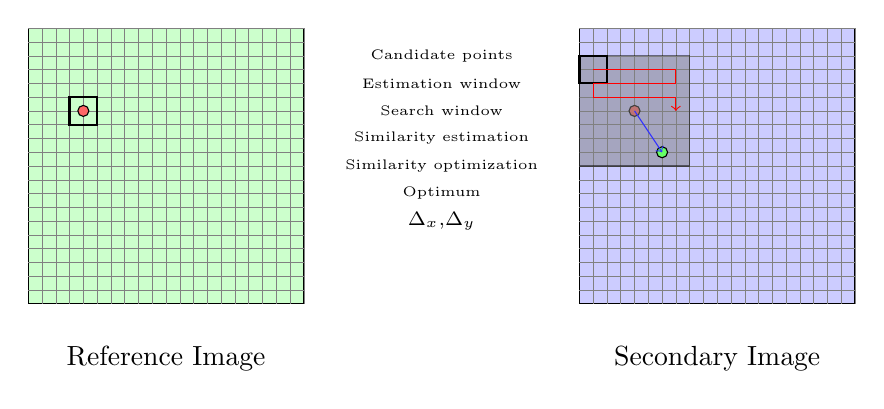
\begin{tikzpicture}[scale=0.35]
    \draw[fill=green!20] (5,5) rectangle (15,15);
    \draw[step=0.5, gray, very thin] (5,5) grid (15,15);
    \node (Reference) at (10,3) {Reference Image};

    \draw[fill=blue!20] (25,5) rectangle (35,15);
    \draw[step=0.5, gray, very thin] (25,5) grid (35,15);
    \node (Reference) at (30,3) {Secondary Image};
    
    \draw[fill=red!60] (7,12) circle (0.2);
    \draw[fill=red!60] (27,12) circle (0.2);
    \node (CPs) at (20,14) {\tiny Candidate points};
    
    \draw[thick] (6.5,11.5) rectangle +(1,1);
    \node (EW) at (20,13) {\tiny Estimation window};
    
    \draw[fill=gray, opacity=0.5] (25,10) rectangle +(4,4);
    \node (SW) at (20,12) {\tiny Search window};
    
    \draw[thick] (25,13) rectangle +(1,1);
    \node (SEW) at (20,11) {\tiny Similarity estimation};
    
    \draw[red,->] (25.5,13.5) --  ++(3,0) -- ++(0,-0.5) -- ++(-3,0) -- ++(0,-0.5) --++(3,0) -- ++(0,-0.5)  ;
    \node (OPT) at (20,10) {\tiny Similarity optimization};
    
    \draw[fill=green!60] (28,10.5) circle (0.2);
    \node (OPTF) at (20,9) {\tiny Optimum};
    
    \draw[blue!80,->] (27,12) -- (28,10.5);
    \node (Deltas) at (20,8) {$\scriptstyle{\Delta_x,\Delta_y}$};
    
  \end{tikzpicture}
    \end{center}
\caption{Estimation of the correlation surface.}
\label{zones}
\end{figure}


That means that for each position we compute the correlation
coefficient. The result is a correlation surface whose
maximum gives the most likely local shift between both images:

\begin{equation}
\begin{split}
&\rho_{I,J}(\Delta x, \Delta y) = \\
&\frac{1}{N}\frac{\sum_{x,y}(I(x,y)-m_I)(J(x+\Delta x,y+\Delta y)-m_J)}{\sigma_I
\sigma_J}.
\end{split}
\end{equation}

In this expression, $N$ is the number of pixels of the analysis
window, $m_I$ and $m_J$ are the estimated mean values inside the
analysis window of respectively image $I$ and image $J$ and $\sigma_I$
and $\sigma_J$ are their standard deviations.\\

Quality criteria can be applied to the estimated maximum in order to
 give a confidence factor to the estimated shift: width of the peak,
 maximum value, etc. Sub-pixel shifts can be measured by applying
 fractional shifts to the sliding window. This can be done by image interpolation.\\

The interesting parameters of the procedure are:
\begin{itemize}
\item The size of the exploration area: it determines the
computational load of the algorithm (we want to reduce it), but it has
to be large enough in order to cope with large deformations.
\item The size of the sliding window: the robustness of the correlation
coefficient estimation increases with the window size, but the
hypothesis of local rigid shifts may not be valid for large windows.
\end{itemize}

The correlation coefficient cannot be used with original grey-level
images in the multi-sensor case. It could be used on extracted
features (edges, etc.), but the feature extraction can introduce
localization errors. Also, when the images come from sensors using
very different modalities, it can be difficult to find similar
features in both images. In this case, one can try to find the
similarity at the pixel level, but with other similarity measures and
apply the same approach as we have just described.\\

The concept of similarity measure has been presented in definition
\ref{def-simil}. The difficulty of the procedure lies in finding the
function $f$ which properly represents the criterion $c$. We also need
that $f$ be easily and robustly estimated with small windows. We extend here what we proposed in \cite{ig02simil}.\\

\subsection{The correlation coefficient\label{expe}}
We remind here the computation of the correlation coefficient between
two image windows $I$ and $J$. The coordinates of the pixels inside
the windows are represented by $(x,y)$:

\begin{equation}
\rho(I,J) = \frac{1}{N}\frac{\sum_{x,y}(I(x,y)-m_I)(J(x,y)-m_J)}{\sigma_I
\sigma_J}.
\label{coeffcorr}
\end{equation}

In order to qualitatively characterize the different similarity
measures we propose the following experiment. We take two images which
are perfectly registered and we extract a small window
of size $N\times M$ from each of the images (this size is set to
$101\times 101$ for this experiment). For the master image, the
window will be centered on coordinates $(x_0,
y_0)$ (the center of the image) and for the slave image, it will be centered on coordinates $(x_0+\Delta x,
y_0)$. With different values of $\Delta x$ (from -10 pixels to 10
pixels in our experiments), we obtain an estimate of $\rho(I,J)$ as a
function of $\Delta x$, which we write as
$\rho(\Delta x)$ for short. The obtained curve should have a maximum for
$\Delta x =0$, since the images are perfectly registered. We would
also like to have an absolute maximum with a high value and with a
sharp peak, in order to have a good precision for the shift estimate.\\

%% In the following, we will make this experiment with different image
%% pairs and different similarity measures. Figure \ref{fig-correl}
%% shows the results obtained when the correlation coefficient is applied
%%  to (\ref{correl-B1B1}) one extract of the B1 channel of a Spot 5
%% image with itself, (\ref{correl-B1B3}) an extract of channel B1 with the
%% extract of channel B3,  and (\ref{correl-B1ERS}) the extract of
%% channel B1 with an
%% extract of an ERS-2 SAR image. The images are presented in figures
%% \ref{histo_b1_b1}, \ref{histo_b1_b3} and \ref{histo_b1_ers}.\\


%% % \begin{figure*}
%% % \centerline{\subfigure[Correlation B1-B1]{\includegraphics[width=0.5\hsize]{CORREL_b1_b1_10.pdf}\label{correl-B1B1}} \\
%% % \subfigure[Correlation
%% % B1-B3]{\includegraphics[width=0.5\hsize]{CORREL_b1_b3_10.pdf}\label{correl-B1B3}}\\
%% % \subfigure[Correlation B1-ERS]{\includegraphics[width=0.5\hsize]{CORREL_b1_ERS_10_0.pdf}\label{correl-B1ERS}}}
%% % \caption{Measure of $\rho(\Delta x)$ for 3 different pairs of images.}
%% % \label{fig-correl}
%% % \end{figure*}

%% \begin{figure*}
%% \centering
%% \subfigure[Correlation B1-B1]{\includegraphics[width=0.4\hsize]{CORREL_b1_b1_10.pdf}\label{correl-B1B1}} \\
%% \subfigure[Correlation
%% B1-B3]{\includegraphics[width=0.4\hsize]{CORREL_b1_b3_10.pdf}\label{correl-B1B3}}\\
%% \subfigure[Correlation B1-ERS]{\includegraphics[width=0.4\hsize]{CORREL_b1_ERS_10_0.pdf}\label{correl-B1ERS}}
%% \caption{Measure of $\rho(\Delta x)$ for 3 different pairs of images.}
%% \label{fig-correl}
%% \end{figure*}

%% We can see that the correlation coefficient has a good behavior for
%% the first pair, but its performances are bad when the images
%% radiometries are different. The correlation coefficient
%%  can be characterized as follows:
%% \begin{itemize}
%% \item Well known algorithm.
%% \item Fits the registration needs when using radiometrically similar images.
%% \item Simple and fast computation.
%% \item High precision in the estimation of the deformation.
%% \item Robust to noise.
%% \end{itemize}

%% However its main disadvantage is that it can only take into account
%%  affine transformations between radiometries ($j = \alpha i + \beta$)
%%  so it can not be used in the general multi-sensor case.\\


%% \subsection{Generalization: probabilistic interpretation \label{sec_correl}}
%% The correlation coefficient formulation (equation \ref{coeffcorr}) can
%% be revisited with a probabilistic interpretation:

%% \begin{equation}
%% \begin{split}
%% \rho(I,J) &= \frac{1}{N}\frac{\sum_{x,y}(I(x,y)-m_I)(J(x,y)-m_J)}{\sigma_I
%% \sigma_J} \\
%% &= \sum_{(i,j)}\frac{(i-m_I)(j-m_J)}{\sigma_I \sigma_J}p_{ij}
%% \end{split}
%% \label{coeffcorr2}
%% \end{equation}

%% where the sum is taken over the list of radiometry pairs $(i,j)$, and
%% $p_{ij}$ is the value of the joint normalized histogram (estimation of
%% the joint probability density function, pdf, $f_{ij}(i,j)$) of the pair of images.\\

%% That means that we are assuming a linear model
%% \begin{equation}
%% j = (i-m_I)\frac{\sigma_J}{\sigma_I}+m_J,
%% \end{equation}
%% and we evaluate its likelihood by weighting with the probability of
%% each radiometry couple, $p_{ij}$.\\

%% One could assume different models for the radiometry pairs leading to
%% different measures as, for instance, the identity model , $i=j$, which
%% leads to the $L_n$ norm:

%% \begin{equation}
%% L_n(I,J) = \sum_{i,j} \left| i - j\right|^n p_{ij},
%% \end{equation}

%% or more complex models based on textural approaches :

%% Diagonal moment:
%% \begin{equation}
%% MD(I,J) = \sum_{i,j}\left| i - j\right|(i+j-\sigma_I-\sigma_J) p_{ij},
%% \end{equation}

%%  Cluster Shade:
%% \begin{equation}
%% C_{shade}(I,J) = \sum_{i,j} (i+j-\sigma_I-\sigma_J)^3 p_{ij},
%% \end{equation}

%%  Cluster Prominence:
%% \begin{equation}
%% C_{pro}(I,J) = \sum_{i,j} (i+j-\sigma_I-\sigma_J)^4 p_{ij}.
%% \end{equation}

%% An assessment of these measures for image registration can be found in
%% \cite{bro}. They are very sensitive to noise and are not useful for
%% the comparison of grey-levels of multi-sensor image pairs.\\

%% \subsection{Estimation of similarity measures and $p_{IJ}$}

%% In the expression of the correlation coefficient the term $p_{ij}$ is
%% an estimation of the joint pdf of the radiometries of
%% the images we are comparing. It can be seen as a link (transfer
%% function) between both radiometries.\\

%% % We want a measure of the
%% % similarity measure which is valid locally, that is, which takes into
%% % account the specificities of the neighborhood of the pixel for which
%% % we are estimating the deformation. That means that we have to use a
%% % small estimation window around the pixel of interest. On the other
%% % hand, we want a robust estimate, thus we need reliable values of
%% % $p_{ij}$, which means the use of a high number of samples.\\


%% %\subsubsection{Examples of $p_{ij}$ estimation}

%% We show here several examples of the estimation of the joint
%% histogram. On figures \ref{histo_b1_b1}, \ref{histo_b1_b3} and
%% \ref{histo_b1_ers} are shown respectively the joint histograms of one
%% image with itself (B1-B1), two different channels of the same Spot 5
%% image (B1-B3) and a Spot 5 B3 - ERS-2 pair.\\

%% \begin{figure}
%% \centering
%% \subfigure[SPOT 5 B1]{\includegraphics[width=0.5\hsize]{b1_1980_1980.pdf}} \\
%% \subfigure[Joint histogram]{\includegraphics[width=0.5\hsize]{hb1.pdf}}
%% \caption{Joint histogram of an image with itself.}
%% \label{histo_b1_b1}
%% \end{figure}


%% \begin{figure}
%% \centering
%% \subfigure[SPOT 5 B1]{\includegraphics[width=0.5\hsize]{b1_3376_3882.pdf}}\\
%% \subfigure[SPOT 5 B3]{\includegraphics[width=0.5\hsize]{b3_3376_3882.pdf}}\\
%% \subfigure[Joint histogram]{\includegraphics[width=0.5\hsize]{hb3.pdf}}\\
%% \caption{Joint histogram of two channels (B1-B3) of the same Spot 5 image.}
%% \label{histo_b1_b3}
%% \end{figure}



%% \begin{figure}
%% \centering
%% \subfigure[SPOT 5 B3]{\includegraphics[width=0.5\hsize]{b1_1500_2500.pdf}}\\
%% \subfigure[ERS-2]{\includegraphics[width=0.5\hsize]{ERS_1500_2500.pdf}}\\
%% \subfigure[Joint histogram]{\includegraphics[width=0.5\hsize]{hers.pdf}}\\
%% \caption{Joint histogram of a Spot 5 B3 image and a ERS-2 image.}
%% \label{histo_b1_ers}
%% \end{figure}

%% As expected, the joint histogram of an image with itself is a straight
%% line with slope 1. It shows the full correlation between the two
%% images: the identity transfer function. This kind of situation is well
%% dealt with by the correlation coefficient.\\

%% The B1-B3 case (figure \ref{histo_b1_b3}) shows two nearly linear tendencies which are
%% mixed up. This case can not be dealt with by the correlation coefficient.\\

%% Finally, figure \ref{histo_b1_ers} shows the impossibility of finding
%% any correlation link between two sensors which are as different as an
%% optical and a radar one.\\


%% \subsubsection{Computation time}
%% The main difference between the two expressions of the correlation
%% coefficient given by equations \ref{coeffcorr} and \ref{coeffcorr2} is
%% the estimation of the joint pdf needed in the second
%% expression. This estimation is usually done by computing the joint
%% histogram. The joint histogram can be computed with different methods,
%% but their discussion is beyond the scope of this paper. However it is
%% important to note that the method chosen for histogram computation may
%% induce significative changes in the computation cost of the similarity
%% measure. As an example, with our implementation (counting with
%% optimization of the number of classes) there is an increase factor of 4 in
%% computation time between equation \ref{coeffcorr} and equation
%% \ref{coeffcorr2}.\\

%% The multi-sensor measures which will be introduced in the next section
%% need the estimation of the joint histogram. Hence, their computation
%% time is comparable to the one of equation \ref{coeffcorr2}. The
%% differences of computation complexity between these measures are
%% negligible, since the longest part of the algorithm is taken by the
%% joint histogram estimation.\\


%% \subsection{Multi-sensor measures.}
%% We introduce here several similarity measures which have been proved
%% useful in the problem of multi-modality medical image registration \cite{dsarrut-thesis}.\\

%% In the following, the sums will be computed over radiometry values. We
%% will use the conditional mean:
%% \begin{equation}
%% m_{I|j} = \frac{1}{p_j}\sum_i i p_{ij};
%% \end{equation}

%% and the conditional variance:

%% \begin{equation}
%% \sigma^2_{I|j} = \frac{1}{p_j}\sum_i (i-m_{I|j})^2 p_{ij}.
%% \end{equation}

%% For each of the following measures, we will perform the experiment
%% described in section \ref{expe}.\\


%% \subsubsection{Measures using the radiometry values and the probabilities}

%% Within this class, we will not take into account the measures which
%% are based on the differences of radiometries ($L_n$ norm of the
%% difference) \cite{tru98,cm87,akn89}, or textural measures, since they
%% give low quality results.\\


%% \paragraph{Normalised standard deviation or Woods criterion}

%% The work by Woods et al. first on mono-modal registration 
%% \cite{wcm92} and then on multi-modal registration \cite{wmc93} lead to
%% the elaboration of this similarity measure. Given the intensity on one
%% image, that is the set of pixels having this value, this measure takes
%% into account the variability of the intensities of the homologous
%% pixels in the other image. The underlying hypothesis is that this
%% variability (which is actually a measure of variance) will be minimum
%% when the images are registered:

%% \begin{equation}
%% Woods(I|J) = \sum_j \frac{\sigma_{I|j}}{m_{I|j}}p_j
%% \end{equation}

%% In order to have a criterion which has to be maximised, we will use:
%% \begin{equation}
%% S_{Woods}(I|J) = 1-\sum_j \frac{\sigma_{I|j}}{m_{I|j}}p_j
%% \end{equation}

%% The results on our three test image pairs are shown in figure
%% \ref{woods}. We see that for the mono-sensor case the results are
%% similar to those of the correlation coefficient. For the two
%% multi-sensor examples, we obtain high values near the 0-shift, but the
%% location of these maxima is not accurate.\\

%% \begin{figure*}
%% \centering
%% \subfigure[B1 with B1]{\includegraphics[width=0.4\hsize]{WOODS_b1_b1_1_60_15.pdf}}\\
%% \subfigure[B1 with B3]{\includegraphics[width=0.4\hsize]{WOODS_b1_b3_1_60_15.pdf}}\\
%% \subfigure[B1 with ERS]{\includegraphics[width=0.4\hsize]{WOODS_b1_ERS_60_15_0.pdf}}
%% \caption{Image shift experiment: Woods criterion.}
%% \label{woods}
%% \end{figure*}


%% \paragraph{Correlation ratio}

%% This is a very well known measure in statistics. It has been first
%% proposed in the framework of image registration by Roche et
%% al. \cite{rmpa98b}. It is defined as follows:
%% \begin{equation}
%% \eta^2(I|J) = 1-\frac{1}{\sigma_I^2}\sum_j \sigma_{I|j}^2p_j
%% \end{equation}

%% Its interpretation is similar to the one of the Woods criterion. The
%% results are shown in figure \ref{rapcorr} and they are worse than
%% those of the Woods criterion.\\

%% \begin{figure*}
%% \centering
%% \subfigure[B1 with B1]{\includegraphics[width=0.4\hsize]{RAPCORR_b1_b1_0_80_10.pdf}}\\
%% \subfigure[B1 with B3]{\includegraphics[width=0.4\hsize]{RAPCORR_b1_b3_1_60_10.pdf}}\\
%% \subfigure[B1 with ERS]{\includegraphics[width=0.4\hsize]{RAPCORR_b1_ERS_80_10_0.pdf}}
%% \caption{Image shift experiment: Correlation ratio.}
%% \label{rapcorr}
%% \end{figure*}

%% \subsubsection{Measures using only the probabilities}

%% This class of measures does not directly use the radiometries of the
%% pixels, but only the estimation of the joint pdf. Of course,
%% the pixel pairs are used for the estimation of this probability.\\


%% \paragraph{Distance to independence}

%% It is a normalised version of the $\chi^2$ test:
%% \begin{equation}
%% \chi^2(I,J) = \sum_{i,j}\frac{(p_{ij}-p_i p_j)^2}{p_i p_j}
%% \end{equation}

%% It measures the degree of statistical dependence between both images,
%% since for two independent random variables, the joint pdf is
%% equal to the product of the marginals. The correlation coefficient is
%% a test of independence of order 2 and this one is the generalisation
%% to any order. The results are shown in figure \ref{chi2}. In this
%% case, for the three pairs, we obtain an absolute maximum for the
%% 0-shift case which is sharp enough for a robust automatic detection.\\

%% \begin{figure*}
%% \centering
%% \subfigure[B1 with B1]{\includegraphics[width=0.4\hsize]{KI2_b1_b1_0_100_5.pdf}}\\
%% \subfigure[B1 with B3]{\includegraphics[width=0.4\hsize]{KI2_b1_b3_1_100_5.pdf}}\\
%% \subfigure[B1 with ERS]{\includegraphics[width=0.4\hsize]{KI2_b1_ERS_100_5_0.pdf}}
%% \caption{Image shift experiment: Distance to independence.}
%% \label{chi2}
%% \end{figure*}


%% \paragraph{The $f-divergence$ family}
%% A $f-divergence$ \cite{csiszar} measures the expectation of the
%% diversity of the likelihood ratio between two distributions $P$ and $Q$:

%% \begin{equation}
%% \begin{split}
%% D_{f}(P,Q) = E_Q \left[f\left( \frac{d p(x)}{d q(x)} \right)\right] 
%% =  \int f\left(\frac{p(x)}{q(x)}\right)q(x) dx
%% \end{split}
%% \end{equation}

%% $E_Q$ is the expectation with respect to $Q$, $\frac{d p(x)}{d q(x)}$
%% is the derivative with respect to a density, 
%% $f$ is continuous and convex on $[0,+\infty)$. A divergence can be
%% seen as a relative entropy. In order to simplify the
%% notation, we will use: $p=p_{ij}$, $q=p_i p_j$, $\int = \sum_{i,j}$.\\


%% \begin{table}[b]
%% \begin{center}
%% \begin{tabular}{|c|c|}
%% \hlx{hv}
%% Measure & $f(x)$ \\
%% \hlx{hv}
%% Kolmogorov distance & $\frac{1}{2}|x-1|$ \\
%% \hlx{hv}
%% Mutual information & $x\log x$ \\
%% \hlx{hv}
%% Kullback divergence & $(x-1)\log x$ \\
%% \hlx{hv}
%% $\chi^2$-divergence & $\frac{1}{2}(x -1)^2$ \\
%% \hlx{hv}
%% Hellinger distance & $\frac{1}{2}(\sqrt x -1)^2$ \\
%% % \hlx{hv}
%% % Bhattacharyaa distance & $\sqrt x$ \\
%% \hlx{hv}
%% Toussaints distance & $x \frac{x-1}{x+1}$ \\
%% \hlx{hv}
%% Lin K-divergence & $x\log \frac{2x}{1+x}$ \\
%% \hlx{vhs}
%% \end{tabular}
%% \end{center}
%% \caption{Expressions of function $f$ in the $f-divergence$ family.}
%% \label{tabfg}
%% \end{table}

%% Depending on the choice of $f$ (see table \ref{tabfg}), we can obtain several
%% interesting cases:


%% \begin{enumerate}
%% \item Kolmogorov distance:
%% \begin{equation}
%% V(P,Q) = \frac{1}{2} \int\left| p -q\right|
%% \end{equation}


%% \item Kullback information or mutual information:
%% \begin{equation}
%% K(P,Q) = \int p \log\frac{p}{q}
%% \end{equation}


%% \item Kullback divergence:
%% \begin{equation}
%% K'(P,Q) = \int (q-p)\left( \log q - \log p \right)
%% \end{equation}

%% \item $\chi^2$-divergence:
%% \begin{equation}
%% R(P,Q) = \frac{1}{2}\int \frac{(p-q)^2}{q}
%% \end{equation}


%% \item Hellinger distance:
%% \begin{equation}
%% {\cal H}^2 (P,Q) = \frac{1}{2}\int (\sqrt p - \sqrt q)^2
%% \end{equation}

%% % \item Bhattacharyaa distance:
%% % \begin{equation}
%% % {\cal B} (P,Q) = -2 \log\left(\int \sqrt{ p q}\right)
%% % \end{equation}

%% \item Toussaints distance:
%% \begin{equation}
%% T (P,Q) = \int p-\frac{2pq}{p+q}
%% \end{equation}


%% \item Lin K-divergence:
%% \begin{equation}
%% K_{div} (P,Q) = \int p\log \frac{2p}{p+q}
%% \end{equation}

%% \end{enumerate}


%% All these measures give very similar results \cite{sm99}. We study two of them:



%% \begin{enumerate}
%% \item Kolmogorov distance
%% \begin{equation}
%% V(P,Q) = \frac{1}{2} \int\left| p_{ij} -p_i p_j\right|
%% \end{equation}

%% It can be seen as a $L_1$ norm version of the $\chi^2$ criterion. The
%% results are shown in figure \ref{distkol}.\\


%% \begin{figure*}
%% \centering
%% \subfigure[B1 with B1]{\includegraphics[width=0.4\hsize]{DISTKOLM_b1_b1_0_100_5.pdf}}\\
%% \subfigure[B1 with B3]{\includegraphics[width=0.4\hsize]{DISTKOLM_b1_b3_1_100_5.pdf}}\\
%% \subfigure[B1 with ERS]{\includegraphics[width=0.4\hsize]{DISTKOLM_b1_ERS_100_5_0.pdf}}
%% \caption{Image shift experiment: Kolmogorov distance.}
%% \label{distkol}
%% \end{figure*}


%% \item Mutual information
%% \begin{equation}
%% K(P,Q) = \int p_{ij} \log\frac{p_{ij}}{p_i p_j}
%% \end{equation}


%% The results are shown in figure \ref{infokull}.\\


%% \begin{figure*}
%% \centering
%% \subfigure[B1 with B1]{\includegraphics[width=0.4\hsize]{INFKULL_b1_b1_0_100_5.pdf}}\\
%% \subfigure[B1 with B3]{\includegraphics[width=0.4\hsize]{INFKULL_b1_b3_1_100_5.pdf}}\\
%% \subfigure[B1 with ERS]{\includegraphics[width=0.4\hsize]{INFKULL_b1_ERS_100_5_0.pdf}}
%% \caption{Image shift experiment: Mutual information.}
%% \label{infokull}
%% \end{figure*}

%% \end{enumerate}


%% Both measures give satisfactory results which are very similar to the
%% ones obtained with the distance to the independence.\\


%% % \paragraph{Proportional reduction of the prediction error}

%% % It is an extension of the correlation concept to categorial variables
%% %  \cite{shh98,weh96,rmap99}. We measure the ability of a variable to
%% %  predict the other. We define an uncertainty measure $V(I)$ and the
%% %  prediction error is defined as:
%% % \begin{equation}
%% % PRE_V(I|J) = \frac{V(I)-E\left[ V(I|J) \right]}{V(I)}
%% % \end{equation}

%% % This measure can be made symmetric:
%% % \begin{equation}
%% % PRE_V(I,J) = \frac{V(I)+V(J)-E\left[ V(I|J) \right]- E\left[ V(J|I) \right]}{V(I)+V(J)}
%% % \end{equation}

%% % If the uncertainty measure used is the entropy, one can define the
%% % following coefficients:
%% % \begin{equation}
%% % u(I|J) = \frac{H(I)-H(I|J)}{H(I)}=\frac{{\cal I}(I,J)}{H(I)}
%% % \end{equation}

%% % \begin{equation}
%% % k(I,J) = \frac{{\cal I}(I,J)}{H(I)+H(J)}
%% % \end{equation}

%% % \begin{equation}
%% % r(I,J) = \sqrt{1-\left( \frac{{\cal I}(I,J)}{H(I,J)} \right)^2}
%% % \end{equation}

%% % With this same principle and using the variance a s uncertainty
%% %  measure we obtain the correlation ratio:
%% % \begin{equation}
%% % \eta^2(I|J) = \frac{Var(I)-Var(E[I|J])}{Var(I)}
%% % \end{equation}

%% % We detail the results of one of these measures:

%% % \paragraph{U criterion}
%% % \begin{equation}
%% % u(I|J) = \frac{H(I)-H(I|J)}{H(I)}=\frac{{\cal I}(I,J)}{H(I)}
%% % \end{equation}

%% % It measures the the entropy and the conditional entropy. This distance
%% % increases when the two variables are linked. The results on our 3 test
%% % pairs are shown on figure \ref{critereU}.\\


%% % \begin{figure*}
%% % \centerline{\subfigure[B1 with B1]{\includegraphics[width=0.5\hsize]{U_b1_b1_1_40.pdf}}\\
%% % \subfigure[B1 with B3]{\includegraphics[width=0.5\hsize]{U_b1_b3_1_40.pdf}}\\
%% % \subfigure[B1 with ERS]{\includegraphics[width=0.5\hsize]{U_b1_ERS_80_0.pdf}}}
%% % \caption{Image shift experiment: U criterion.}
%% % \label{critereU}
%% % \end{figure*}


%% \paragraph{Cluster reward algorithm}


%% Let $H_{IJ}(k,l)$ be the joint histogram of the pair of images and
%% let  $H_I(k)$ and $H_J(k)$ respectively be the marginal histograms and
%% $P$ the number of pixels. We define 
%% \begin{equation}
%% I_{CRA} = \frac{\frac{\Phi}{F}- \frac{F}{P^2}}{1-\frac{F}{P^2}};
%% \label{cra}
%% \end{equation}
 
%% where
%% \begin{subequations}
%% \begin{equation}
%% \Phi = \sum_{k=0}^{N-1} \sum_{l=0}^{N-1} H_{IJ}^2(k,l);
%% \end{equation}
%% \begin{equation}
%% F=\sqrt{h_I h_J};
%% \end{equation}
%% \begin{equation}
%% h_I = \sum_{k=0}^{N-1} H_{I}^2(k);
%% \end{equation}
%% \begin{equation}
%% h_J = \sum_{k=0}^{N-1} H_{J}^2(k);
%% \end{equation}
%% \end{subequations}

%% The $I_{CRA}$ index will have a high value when the joint histogram
%% has little dispersion. This lack of dispersion can be due to a
%% correlation (histogram distributed along a line) or to the clustering
%% of radiometry values within the histogram. In both cases one can
%% predict the values of one image from the values of the other.\\

%% In order to compare $I_{CRA}$ with the $f-divergences$, we can rewrite equation \ref{cra} as:

%% \begin{equation}
%% I_{CRA} = \frac{\int p_{ij}^2 - \int p_i^2
%% \int p_j^2}{\sqrt{\int p_i^2 \int p_j^2} - \int p_i^2
%% \int p_j^2}.
%% \label{cra2}
%% \end{equation}
%%  If we consider the denominator as a normalization term, we can focus
%% only in the numerator. This numerator contains the same terms as the
%% $f-divergences$, that is, a term which depends on the joint
%% pdf and a term which depends on the product of the
%% marginals. We can thus make an interpretation which is similar to the
%% independence tests. As expected, the obtained results (figure
%% \ref{cra_figure}) are similar to those obtained with the $f-divergences$.\\


%% \begin{figure*}
%% \centering
%% \subfigure[B1 with B1]{\includegraphics[width=0.4\hsize]{K_b1_b1_1_40.pdf}}\\
%% \subfigure[B1 with B3]{\includegraphics[width=0.4\hsize]{K_b1_b3_1_40.pdf}}\\
%% \subfigure[B1 with ERS]{\includegraphics[width=0.4\hsize]{K_b1_ERS_80_0.pdf}}
%% \caption{Image shift experiment: Cluster reward algorithm.}
%% \label{cra_figure}
%% \end{figure*}

%% The main interest of the CRA with respect to the $f-divergence$ family
%% is that the joint histogram noise due to estimation has less influence
%% in the similarity measure. This allows us to use smaller estimation
%% windows. The only drawback in doing this is that the peak of the
%% measure will be less sharp.\\


\section{Regular grid disparity map estimation}
\label{sec:SimpleDisparityMapEstimationDense}
%% \ifitkFullVersion
\input{FineRegistrationImageFilterExample.tex}
%% \fi


\input{StereoReconstruction.tex}
\chapter{Orthorectification and Map Projection}\label{sec:Ortho}


\begin{figure}[h]
  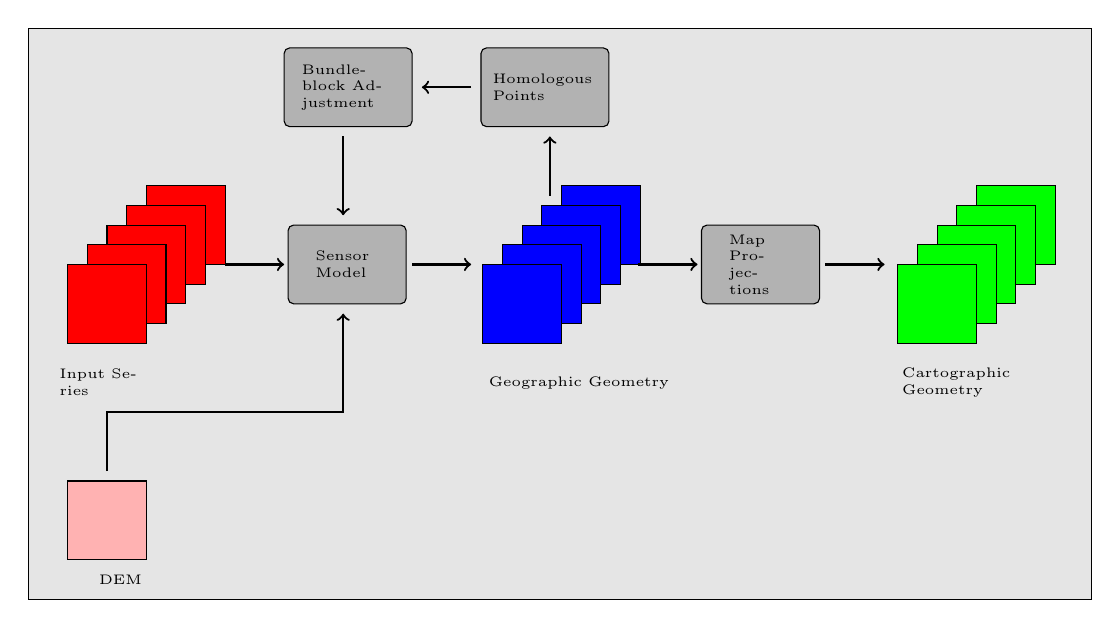
\begin{tikzpicture}[scale=0.25]
    \tiny
    \draw[fill=black!10] (-1,-12) rectangle (53,17);
     \foreach \x in {5,...,1}
       \draw[fill=red] (\x,\x) rectangle +(4,4);
     \node[fill=black!10, text width= 1.2cm] (InputSeries) at
       (3,-1) {Input Series};

     \draw[->,thick] (9,5) --  +(3,0);

     \draw[fill=black!30,rounded corners=2pt] (12.2,3) rectangle +(6,4);
     \node[text width= 0.7cm] (SensorModel) at (15,5) {Sensor Model};

     \draw[fill=red!30] (1,-10) rectangle +(4,4);
     \node[fill=black!10, text width= 1.2cm] (DEM) at
       (5,-11) {DEM};

     \draw[->,thick] (3,-5.5) --  ++(0,3) -- ++(12,0) -- ++(0,5);

     \draw[->,thick] (18.5,5) --  +(3,0);

     \foreach \x in {5,...,1}
       \draw[fill=blue,xshift=600pt] (\x,\x) rectangle +(4,4);
     \node[fill=black!10, text width= 2.8cm] (GeographicGeometry) at
       (28,-1) {Geographic Geometry};



       \draw[->,thick] (25.5,8.5) --  +(0,3);

     \draw[fill=black!30,rounded corners=2pt] (22,12) rectangle +(6.5,4);
     \node[text width= 0.7cm] (HomPoExtr) at (24,14) {Homologous
     Points};

     \draw[->,thick] (21.5,14) --  +(-2.5,0);

     \draw[fill=black!30,rounded corners=2pt] (12,12) rectangle +(6.5,4);
     \node[text width= 1.3cm] (BBAdj) at (15.5,14) {Bundle-block
     Adjustment};

     \draw[->,thick] (15,11.5) --  +(0,-4);


      \draw[->,thick] (30,5) --  +(3,0);

     \draw[fill=black!30,rounded corners=2pt] (33.2,3) rectangle +(6,4);
     \node[text width= 0.7cm] (MapProjection) at (36,5) {Map Projections};



     \draw[->,thick] (39.5,5) --  +(3,0);

     \foreach \x in {5,...,1}
       \draw[fill=green,xshift=1200pt] (\x,\x) rectangle +(4,4);
     \node[fill=black!10, text width= 1.8cm] (CartographicGeometry) at
       (47,-1) {Cartographic Geometry};

     %\draw[->,thick] (36,2) --  ++(0,-10) -- ++(-30,0);

  \end{tikzpicture}
  \itkcaption[Image Ortho-registration Procedure]{Image Ortho-registration Procedure.}
\label{fig:ImageOrtho-registrationProcedure}
\end{figure}

This chapter introduces the functionnalities available in OTB for
image ortho-registration. We define ortho-registration as the
procedure allowing to transform an image in sensor geometry to a
geographic or cartographic projection.\\

Figure \ref{fig:ImageOrtho-registrationProcedure} shows a synoptic
view of the different steps involved in a classical ortho-registration
processing chain able to deal with image series. These steps are the following:
\begin{itemize}
  \item Sensor modelling: the geometric sensor model allows to convert
  image coordinates (line, column) into geographic coordinates
  (latitude, longitude); a rigorous modelling needs a digital
  elevation model (DEM) in order to take into account the terrain
  topography.
  \item Bundle-block adjustment: in the case of image series, the
  geometric models and their parameters can be refined by using
  homologous points between the images. This is an optional step and
  not currently implemented in OTB.
  \item Map projection: this step allows to go from geographic
  coordinates to some specific cartographic projection as Lambert,
  Mercator or UTM.
\end{itemize}


\section{Sensor Models}
\ifitkFullVersion
\label{sec:SensorModels}
\fi

A sensor model is a set of equations giving the relationship between
image pixel $(l,c)$ coordinates and ground $(X,Y)$ coordinates for every
pixel in the image. Typically, the ground coordinates are given in a
geographic projection (latitude, longitude). The sensor model
can be expressed either from image to ground -- forward model -- or
from ground to image -- inverse model. This can be written as follows:

\begin{displaymath}
  \begin{array}{cc}
    Forward & \\
    X = f_x(l,c,h,\vec\theta) & Y = f_y(l,c,h,\vec\theta)\\
     & \\
    Inverse & \\
    l = g_l(X,Y,h,\vec\theta) & c = g_c(X,Y,h,\vec\theta)
  \end{array}
\end{displaymath}

Where $\vec\theta$ is the set of parameters which describe the sensor
and the acquisition geometry (platform altitude, viewing angle, focal
length for optical sensors, doppler centroid for SAR images, etc.).\\

In OTB, sensor models are implemented as \doxygen{itk}{Transform}s
(see section \ref{sec:Transforms} for details), which is the
appropriate way to express coordinate changes. The base class for
sensor models is \doxygen{otb}{SensorModelBase} from which the classes
\doxygen{otb}{InverseSensorModel} and
\doxygen{otb}{ForwardSensorModel} inherit.\\

As one may note from the model equations, the height of the ground, $h$,
must be known. Usually, it means that a Digital Elevation Model,
DEM, will be used.\\


\subsection{Types of Sensor Models}
\label{sec:TypesofSensorModels}
There exists two main types of sensor models. On one hand, we have the
so-called {\em physical models}, which are rigorous, complex,
eventually highly non-linear equations of the sensor geometry. As
such, they are difficult to inverse (obtain the inverse model from the
forward one and vice-versa). They have the significant advantage of having
parameters with physical meaning (angles, distances, etc.). They are
specific of each sensor, which means that a library of models is
required in the software. A library which has to be updated every time a new
sensor is available.\\

On the other hand, we have general analytical models, which
approximate the physical models. These models can take the form of
polynomials or ratios of polynomials, the so-called rational
polynomial functions or Rational Polynomial Coefficients, RPC, also
known as {\em Rapid Positioning Capability}.
Since they are approximations, they are less accurate than the
physical models. However, the achieved accuracy is usually high: in
the case of Pl\'eiades, RPC models have errors lower than 0.02 pixels
with respect to the physical model. Since these models have a standard
form they are easier to use and implement. However, they have the
drawback of having parameters (coefficients, actually) without
physical meaning.\\

OTB, through the use of the OSSIM library --
\url{http://www.ossim.org} -- offers models for most of current
sensors either through a physical or an analytical approach. This is
transparent for the user, since the geometrical model for a given
image is instantiated using the information stored in its meta-data. The 
search for a sensor model is not straightforward. It is done in several steps :
\begin{enumerate}
  \item Load an external \code{.geom} file specified through extended filenames
(if present)
  \item Load the \code{.geom} file attached with the input image (if present).
They share the same name, without extension.
  \item Search in the OSSIM plugin factory for a suitable model 
(\code{ossimplugins::ossimPluginProjectionFactory}). For instance, this
factory contains Pl\'eiades and TerraSar sensor models.
  \item If no model was found, search in the OSSIM projection factory 
(\code{ossimProjectionFactoryRegistry}). For instance this factory contains
Spot5, Landsat and Quickbird sensor models.
  \item If no model was found, search any RPC tags in the input image. When the
tags are present, an \code{ossimRpcModel} is created.
  \item If still no model was found, search for a valid sensor model in other
files attached to the current dataset. For instance, with a Sentinel 1 SAFE
dataset, it will inspect underlying \code{.tiff} files. With a VRT dataset, it
will inspect the files referenced by the VRT.
\end{enumerate}

Note that the \code{.geom} metadata file can store any sensor model recognized
by OSSIM.

\subsection{Using Sensor Models}
\label{sec:UsingSensorModels}

The transformation of an image in sensor geometry to geographic
geometry can be done using the following steps.
  \begin{enumerate}
    \item Read image meta-data and instantiate the model with the
    given parameters.
  \item Define the ROI in ground coordinates (this is your output
  pixel array)
  \item Iterate through the pixels of coordinates $(X,Y)$:
    \begin{enumerate}
      \item Get $h$ from the DEM
      \item Compute $(c,l) = G(X,Y,h,\vec\theta)$
      \item Interpolate pixel values if $(c,l)$ are not grid coordinates.
    \end{enumerate}
  \end{enumerate}

Actually, in OTB, you don't have to manually instantiate the sensor
model which is appropriate to your image. That is, you don't have to
manually choose a SPOT5 or a Quickbird sensor model. This task is
automatically performed by the \doxygen{otb}{ImageFileReader} class in
a similar way as the image format recognition is done. The appropriate
sensor model will then be included in the image meta-data, so you can
access it when needed.

\ifitkFullVersion
\input{SensorModelExample.tex}
\fi

\subsection{Evaluating Sensor Model}
\label{sec:EvaluatingSensorModels}

If no appropriate sensor model is available in the image meta-data,
OTB offers the possibility to estimate a sensor model from the image.

\input{EstimateRPCSensorModelExample.tex}


\subsection{Limits of the Approach}
\label{LimitsoftheApproach}

As you may understand by now, accurate geo-referencing needs accurate
DEM and also accurate sensor models and parameters. In the case where
we have several images acquired over the same area by different
sensors or different geometric configurations, geo-referencing (geographical coordinates) or ortho-rectification
(cartographic coordinates) is not usually enough. Indeed, when working
with image series we usually want to compare them (fusion, change
detection, etc.) at the pixel level.\\

Since common DEM and sensor parameters do not allow for such an
accuracy, we have to use clever strategies to improve the
co-registration of the images. The classical one consists in refining
the sensor parameters by taking homologous points between the images
to co-register. This is called bundle block adjustment and will be
implemented in coming versions of OTB.

Even if the model parameters are refined, errors due to DEM accuracy
can not be eliminated. In this case, image to image registration can
be applied. These approaches are presented in chapters
\ref{chap:ImageRegistration} and \ref{sec:DisparityMapEstimation}.

%% \section{Bundle-block adjustment}
%% Problem position
%%   \begin{itemize}
%%     \item The image series is geo-referenced (using the available DEM,
%%     and the prior sensor parameters).
%%     \item We assume that homologous points (GCPs, etc.) can be easily
%%     obtained from the geo-referenced series : $HP_i = (X_i,Y_i,h_i)$
%%     \item For each image, and each point, we can write:
%%     $(l_{ij},c_{ij}) = G_j(X_i,Y_i,h_i,\vec\theta_j)$
%%   \end{itemize}

%% \begin{tikzpicture}[scale=0.15]
%% \draw[fill=yellow!20] (-5.5,-15.5) rectangle (5.5,-5.5);
%%     \draw[step=0.5, gray, very thin] (-5.5,-15.5) grid (5.5,-5.5);

%%     \draw[fill=green!20,rotate=10] (-15.5,0.5) rectangle (-5.5,10.5);
%%     \draw[step=0.5, gray, very thin,rotate=10] (-15.5,0.5) grid>
%%     (-5.5,10.5);

%%     \draw[fill=blue!20,rotate=-10] (5.5,0.5) rectangle (15.5,10.5);
%%     \draw[step=0.5, gray, very thin,rotate=-10] (5.5,0.5) grid
%%     (15.5,10.5);


%%     \draw[fill=red!70] (1,-11) circle (0.2);

%%     \draw (1,-11) .. controls +(30:1cm) and +(60:1cm) .. (-10,7);

%%     \draw[fill=red!70] (-10,7) circle (0.2);

%%     \node (eq1) at (-12.2,-4) {$\scriptstyle{G_1(X_i,Y_i,h_i,\vec\theta_1)}$};

%%     \draw (1,-11) .. controls +(-30:1cm) and +(-60:1cm) .. (10,7);

%%     \draw[fill=red!70] (10,7) circle (0.2);

%%     \node (eq2) at (7.2,-3) {$\scriptstyle{G_2(X_i,Y_i,h_i,\vec\theta_2)}$};

%% \end{tikzpicture}
%% \begin{itemize}
%%       \item Everything is known.
%% \end{itemize}



%% Model refinement
%%   \begin{itemize}
%%     \item If we define $\vec\theta_j^R = \vec\theta_j +
%%     \vec{\Delta\theta_j}$ as the refined parameters,
%%     $\vec{\Delta\theta_j}$ are the unknowns of the model refinement
%%     problem.
%%     \item We have much more equations than unknowns if enough HPs are
%%     found.
%%     \item We solve using non-linear least squares estimation.
%%       \begin{itemize}
%% 	\item The derivatives of the sensor model with respect to its
%% 	parameters are needed.
%%       \end{itemize}
%%   \end{itemize}


%% Homologous point extraction
%% From manual to automatic procedures
%% \begin{itemize}
%%   \item Manual extraction can be used for a few images and for a few
%%   points
%%   \item We are interested in many images (long time series) and many
%%   points (in order to reduce registration errors)
%%   \item Proposed procedure
%%     \begin{enumerate}
%%       \item Choose candidate points
%%       \item Define a similarity measure
%%       \item Optimize the measure
%%     \end{enumerate}
%% \end{itemize}

%% Salient points
%% Similarity measures


\section{Map Projections}
\ifitkFullVersion
\label{sec:MapProjections}
\fi

Map projections describe the link between geographic coordinates and
cartographic ones. So map projections allow to represent a 2-dimensional manifold of a
3-dimensional space (the Earth surface) in a 2-dimensional space (a
map which used to be a sheet of paper!). This geometrical
transformation doesn't have a unique solution, so over the cartography
history, every country or region in the world has been able to express
the belief of being the center of the universe. In other words, every
cartographic projection tries to minimize the distortions of the 3D to
2D transformation for a given point of the Earth surface\footnote{We
  proposed to optimize an OTB map projection for Toulouse, but we
  didn't get any help from OTB users.}.

In OTB the \doxygen{otb}{MapProjection} class is derived from the
\doxygen{itk}{Transform} class, so the coordinate transformation
points are overloaded with map projection equations. The
\doxygen{otb}{MapProjection} class is templated over the type of
cartographic projection, which is provided by the OSSIM library. In
order to hide the complexity of the approach, some type definitions
for the more common projections are given in the file
\code{otbMapProjections.h} file.

Sometimes, you don't know at compile time what map projection you will need in
your application. In this case, the \doxygen{otb}{GenericMapProjection}
allow you to set the map projection at run-time by passing the WKT identification
for the projection.

\input{MapProjectionExample.tex}

You will seldom use a map projection by itself, but rather in an
ortho-rectification framework. An example is given in the next section.




\section{Orthorectification with OTB}
\ifitkFullVersion
\label{sec:OrthorectificationwithOTB}
\fi
\input{OrthoRectificationExample.tex}

\section{Vector data projection manipulation}
\ifitkFullVersion
\label{sec:VectorDataProjection}
\fi
\input{VectorDataProjectionExample.tex}

\section{Geometries projection manipulation}
\ifitkFullVersion
\label{sec:GeometriesProjection}
\fi
\input{GeometriesProjectionExample.tex}

\section{Elevation management with OTB}
\input{DEMHandlerExample.tex}

\section{Vector data area extraction}
\ifitkFullVersion
\label{sec:VectorDataAreaExtraction}
\fi
\input{VectorDataExtractROIExample.tex}

\input{Radiometry.tex}
\input{Fusion.tex}
\chapter{Feature Extraction}

% \section{Introduction}

Under the term {\em Feature Extraction} we include several techniques
aiming to detect or extract information of low level of abstraction
from images. These {\em features} can be objects : points, lines,
etc. They can also be measures : moments, textures, etc.

\section{Textures}
\subsection{Haralick Descriptors}

This example illustrates the use of the \doxygen{otb}{ScalarImageToTexturesFilter},
which compute the standard Haralick's textural features~\cite{Haralick1973} presented in table~\ref{tab:haralickStandardFeatures},
where $\mu_t$ and $\sigma_t$ are the mean and standard deviation of the row
(or column, due to symmetry) sums, $ \mu =  $ (weighted pixel average)
$ = \sum_{i,j}i \cdot g(i, j) =\sum_{i,j}j \cdot g(i, j) $ due to matrix summetry, and
$ \sigma =  $ (weighted pixel variance) $ = \sum_{i,j}(i - \mu)^2 \cdot g(i, j) =\sum_{i,j}(j - \mu)^2 \cdot g(i, j)  $
due to matrix symmetry.

\begin{table}
\begin{center}
\begin{tabular}{|c|c|}
\hline
& \\
Energy & $ f_1 = \sum_{i,j}g(i, j)^2 $ \\
& \\
\hline
& \\
Entropy & $ f_2 = -\sum_{i,j}g(i, j) \log_2 g(i, j)$, or 0 if $g(i, j) = 0$ \\
& \\
\hline
& \\
Correlation & $ f_3 = \sum_{i,j}\frac{(i - \mu)(j - \mu)g(i, j)}{\sigma^2} $ \\
& \\
\hline
& \\
Difference Moment &  $f_4 = \sum_{i,j}\frac{1}{1 + (i - j)^2}g(i, j) $ \\
& \\
\hline
& \\
Inertia (a.k.a. Contrast) & $ f_5 = \sum_{i,j}(i - j)^2g(i, j) $ \\
& \\
\hline
& \\
Cluster Shade & $ f_6 = \sum_{i,j}((i - \mu) + (j - \mu))^3 g(i, j) $ \\
& \\
\hline
Cluster Prominence & $ f_7 = \sum_{i,j}((i - \mu) + (j - \mu))^4 g(i, j) $ \\
& \\
\hline
& \\
Haralick's Correlation & $ f_8 = \frac{\sum_{i,j}(i, j) g(i, j) -\mu_t^2}{\sigma_t^2} $ \\
& \\
\hline
\end{tabular}
\itkcaption[Haralick features]{Haralick features~\cite{Haralick1973} available in \doxygen{otb}{ScalarImageToTexturesFilter}}
\end{center}
\label{tab:haralickStandardFeatures}
\end{table}

More features are available in \doxygen{otb}{ScalarImageToAdvancedTexturesFilter}.
\relatedClasses
\begin{itemize}
\item \doxygen{otb}{ScalarImageToAdvancedTexturesFilter}
\item \doxygen{otb}{ScalarImageToPanTexTextureFilter}
\item \doxygen{otb}{GreyLevelCooccurrenceIndexedList}
\end{itemize}

\input{TextureExample}

\subsection{PanTex}
\input{PanTexExample}

\subsection{Structural Feature Set}
\input{SFSExample}

\section{Interest Points}
\subsection{Harris detector}
\input{HarrisExample}
\subsection{SIFT detector}
\label{sec:SIFTDetector}
% \input{SIFTFastExample}
\InputIfFileExists{SIFTFastExample.tex}{}{}
\subsection{SURF detector}
\input{SURFExample}

\section{Alignments}
\label{sec:Alignments}
\input{AlignmentsExample}
\section{Lines}
\label{sec:LineDetectors}

\subsection{Line Detection}
\label{sec:LineDetection}
\input{RatioLineDetectorExample}
\input{CorrelationLineDetectorExample}
\input{AsymmetricFusionOfLineDetectorExample}
\input{ParallelLineDetectionExample}


\subsection{Segment Extraction}
\label{sec:SegmentExtraction}
\subsubsection{Local Hough Transform}
\input{LocalHoughExample}
%\input{ExtractSegmentsByStepsExample}
%\input{ExtractSegmentsExample}

\subsubsection{Line Segment Detector}
\label{sec:LSD}
\input{LineSegmentDetectorExample}
\subsection{Right Angle Detector}
\label{sec:RightAngleDetector}
\input{RightAngleDetectionExample}


\section{Density Features}
An interesting approach to feature extraction consists in computing
the density of previously detected features as simple edges or
interest points.
\subsection{Edge Density}
\input{EdgeDensityExample}
\subsection{SIFT Density}
\InputIfFileExists{SIFTDensityExample.tex}{}{}

% \input{SIFTDensityExample}

\section{Geometric Moments}

\subsection{Complex Moments}
\label{sec:ComplexMoments}
The complex geometric moments are defined as:
\begin {equation}
c_{pq} = \int\limits_{-\infty}^{+\infty}\int\limits_{-\infty}^{+\infty}(x + iy)^p(x- iy)^qf(x,y)dxdy,
\label{2.2}
\end{equation}
where $x$ and $y$ are the coordinates of the image $f(x,y)$, $i$ is the
imaginary unit and
$p+q$ is the order of $c_{pq}$. The geometric moments are
particularly useful in the case of scale changes.

\subsubsection{Complex Moments for Images}
\input{ComplexMomentsImageFunctionExample}
\subsubsection{Complex Moments for Paths}
\input{ComplexMomentPathExample}

\subsection{Hu Moments}
\label{sec:HuMoments}
Using the algebraic moment theory, H. Ming-Kuel obtained a family of 7
invariants with respect to planar transformations called Hu invariants,
\cite{hu}. Those invariants can be seen as nonlinear combinations of
the complex moments. Hu invariants have
been very much used in object recognition during the last 30 years,
since they are invariant to rotation, scaling and translation. \cite{flusserinv} gives their expressions :

\begin{equation}
\begin{array}{cccc}
\phi_1 = c_{11};& \phi_2 = c_{20}c_{02};& \phi_3 = c_{30}c_{03};& \phi_4 = c_{21}c_{12};\\
\phi_5 = Re(c_{30}c_{12}^3);& \phi_6 = Re(c_{21}c_{12}^2);& \phi_7 = Im(c_{30}c_{12}^3).&\\
\end{array}
\end{equation}


\cite{dudani} have used these invariants for the recognition of
aircraft silhouettes. Flusser and Suk have used them for image
registration, \cite{flusser_2}.

\subsubsection{Hu Moments for Images}
\input{HuMomentsImageFunctionExample}
%\subsubsection{Hu Moments for Paths}
%\input{HuMomentPathExample}


\subsection{Flusser Moments}
\label{sec:FlusserMoments}
The Hu invariants have been modified and
improved by several authors. Flusser used these moments in order to
produce a new family of descriptors of order higher than 3,
\cite{flusserinv}. These descriptors are invariant to scale and
rotation. They have the following expressions:
\begin {equation}
\begin{array}{ccc}
\psi_1  = c_{11} = \phi_1; &  \psi_2  = c_{21}c_{12} = \phi_4; & \psi_3  = Re(c_{20}c_{12}^2) = \phi_6;\\
\psi_4  = Im(c_{20}c_{12}^2); & \psi_5  = Re(c_{30}c_{12}^3) = \phi_5;
& \psi_6  = Im(c_{30}c_{12}^3) = \phi_7.\\
\psi_7  = c_{22}; & \psi_8  = Re(c_{31}c_{12}^2); & \psi_9  = Im(c_{31}c_{12}~2);\\
\psi_{10} = Re(c_{40}c_{12}^4); & \psi_{11} = Im(c_{40}c_{12}^2). &\\

\end{array}
\end {equation}

\textbf{Examples}
\subsubsection{Flusser Moments for Images}
\input{FlusserMomentsImageFunctionExample}
%\subsubsection{Flusser Moments for Paths}
%\input{FlusserMomentPathExample}

\section{Road extraction}
\label{sec:RoadExtraction}

Road extraction is a critical feature for an efficient use of high resolution satellite images. There are many applications of road extraction: update of GIS database, reference for image registration, help for identification algorithms and rapid mapping for example.  Road network can be used to register an optical image with a map or an optical image with a radar image for example. Road network extraction can help for other algorithms: isolated building detection, bridge detection. In these cases, a rough extraction can be sufficient. In the context of response to crisis, a fast mapping is necessary: within 6~hours, infrastructures for the designated area are required. Within this timeframe, a manual extraction is inconceivable and an automatic help is necessary.

\subsection{Road extraction filter}

\input{ExtractRoadExample}

\subsection{Step by step road extraction}

\input{ExtractRoadByStepsExample}


% \section{Seam carving}
% \label{sec:SeamCarving}
%
% \input{SeamCarvingExample}
%
% \input{SeamCarvingOtherExample}

\section{Cloud Detection}
\input{CloudDetectionExample}

\input{ImageSimulation.tex}
\input{DimensionReduction.tex}
\chapter{Classification}

\section{Introduction}

Image classification consists in extracting added-value information from images. 
Such processing methods classify pixels within images into geographical connected 
zones with similar properties, and identified by a common class label. The 
classification can be either unsupervised or supervised.

Unsupervised classification does not require any additional information about the
properties of the input image to classify it. On the contrary, supervised methods 
need a preliminary learning to be computed over training datasets having similar 
properties than the image to classify, in order to build a classification model.

\section{Machine Learning Framework}

\subsection{Machine learning models}
\label{sec:MLGenericFramework}

The OTB classification is implemented as a generic Machine Learning
framework, supporting several possible machine learning libraries as backends.
The base class \doxygen{otb}{MachineLearningModel} defines this framework.
As of now libSVM (the machine learning library historically integrated in OTB),
machine learning methods of OpenCV library (\cite{opencv_library}) and also
Shark machine learning library (\cite{shark_library}) are available. Both
supervised and unsupervised classifiers are supported in the framework.

The current list of classifiers available through the same generic interface within the OTB is:

\begin{itemize}
  \item \textbf{LibSVM}: Support Vector Machines classifier based on libSVM.
  \item \textbf{SVM}: Support Vector Machines classifier based on OpenCV, itself based on libSVM.
  \item \textbf{Bayes}: Normal Bayes classifier based on OpenCV.
  \item \textbf{Boost}: Boost classifier based on OpenCV.
  \item \textbf{DT}: Decision Tree classifier based on OpenCV.
  \item \textbf{RF}: Random Forests classifier based on the Random Trees in OpenCV.
  \item \textbf{KNN}: K-Nearest Neighbors classifier based on OpenCV.
  \item \textbf{ANN}: Artificial Neural Network classifier based on OpenCV.
  \item \textbf{SharkRF} : Random Forests classifier based on Shark.
  \item \textbf{SharkKM} : KMeans unsupervised classifier based on Shark.
\end{itemize}

These models have a common interface, with the following major functions:
\begin{itemize}
  \item \code{SetInputListSample(InputListSampleType *in)} : set the list of input samples
  \item \code{SetTargetListSample(TargetListSampleType *in)} : set the list of target samples
  \item \code{Train()} : train the model based on input samples
  \item \code{Save(...)} : saves the model to file
  \item \code{Load(...)} : load a model from file
  \item \code{Predict(...)} : predict a target value for an input sample
  \item \code{PredictBatch(...)} : prediction on a list of input samples
\end{itemize}

The \code{PredictBatch(...)} function can be multi-threaded when
called either from a multi-threaded filter, or from a single location. In
the later case, it creates several threads using OpenMP.
There is a factory mechanism on top of the model class (see
\doxygen{otb}{MachineLearningModelFactory}). Given an input file,
the static function \code{CreateMachineLearningModel(...)} is able
to instantiate a model of the right type.

For unsupervised models, the target samples \textbf{still have to be set}. They
won't be used so you can fill a ListSample with zeros.

%-------------------------------------------------------------------------------
\subsection{Training a model}

The models are trained from a list of input samples, stored in a
\subdoxygen{itk}{Statistics}{ListSample}. For supervised classifiers, they
also need a list of targets associated to each input sample. Whatever the
source of samples, it has to be converted into a \code{ListSample} before
being fed into the model.

Then, model-specific parameters can be set. And finally, the \code{Train()}
method starts the learning step. Once the model is trained it can be saved
to file using the function \code{Save()}. The following examples show how
to do that.

\input{TrainMachineLearningModelFromSamplesExample.tex}

\input{TrainMachineLearningModelFromImagesExample.tex}

%-------------------------------------------------------------------------------
\subsection{Prediction of a model}

For the prediction step, the usual process is to:
\begin{itemize}
\item Load an existing model from a file.
\item Convert the data to predict into a \code{ListSample}.
\item Run the \code{PredictBatch(...)} function.
\end{itemize}

There is an image filter that perform this step on a whole image, supporting
streaming and multi-threading: \doxygen{otb}{ImageClassificationFilter}.

\ifitkFullVersion
\input{SupervisedImageClassificationExample.tex}
\fi

%-------------------------------------------------------------------------------
\subsection{Integration in applications}

The classifiers are integrated in several OTB Applications. There is a base
class that provides an easy access to all the classifiers:
\subdoxygen{otb}{Wrapper}{LearningApplicationBase}. As each machine learning
model has a specific set of parameters, the base class
\code{LearningApplicationBase} knows how to expose each type of classifier with
its dedicated parameters (a task that is a bit tedious so we want to implement
it only once). The \code{DoInit()} method creates a choice parameter named
\code{classifier} which contains the different supported classifiers along
with their parameters.

The function \code{Train(...)} provide an easy way to train the selected
classifier, with the corresponding parameters, and save the model to file.

On the other hand, the function \code{Classify(...)} allows to load a model
from file and apply it on a list of samples.

%%%%%%%%%%%%%%%%%%%%%%%%%%%%%%%%%%%%%%%%%%%%%%%%%%%%%%%%%%%%%%%%%%%%%%%%%%%%%%%%
\section{Supervised classification}

\subsection{Support Vector Machines}
\label{sec:SupportVectorMachines}

\subsubsection{SVM general description}
Kernel based learning methods in general and the Support Vector
Machines (SVM) in particular, have been introduced in the last years
in learning theory for classification and regression tasks,
\cite{vapnik}. SVM have been successfully applied to text
categorization, \cite{joachims}, and face recognition,
\cite{osuna}. Recently, they have been successfully used for the
classification of hyperspectral remote-sensing images, \cite{bruzzoneSVM}.

Simply stated, the approach consists in searching for the separating
surface between 2 classes by the determination of the subset of
training samples which best describes the boundary between the 2
classes. These samples are called support vectors and completely
define the classification system. In the case where the two classes are
nonlinearly separable, the method uses a kernel expansion in order to make
projections of the feature space onto higher dimensionality spaces
where the separation of the classes becomes linear.


\subsubsection{SVM mathematical formulation}

This subsection reminds the basic principles of SVM learning and
classification. A good tutorial on SVM can be found in, \cite{burges}.
 
We have $N$ samples represented by the couple $(y_i,\mathbf{x}_i),
i=1\ldots N$ where $y_i \in \{-1,+1\}$ is the class label and
$\mathbf{x}_i \in \mathbb{R}^n$ is the feature vector of dimension
$n$. A classifier is a function  $$f(\mathbf{x},\boldsymbol{\alpha}) :
\mathbf{x}\mapsto y$$ where $\boldsymbol{\alpha}$ are the classifier
parameters. The SVM finds the optimal separating hyperplane which
fulfills the following constraints :
    \begin{itemize}
      \item The samples with labels $+1$ and $-1$ are on different
      sides of the hyperplane.
      \item The distance of the closest vectors to the hyperplane is
      maximised. These are the support vectors (SV) and this distance is
      called the margin.
    \end{itemize}

    The separating hyperplane has the equation
    $$\mathbf{w}\cdot\mathbf{x}+b=0;$$ with $\mathbf{w}$ being its
    normal vector and $x$ being any point of the hyperplane. The
    orthogonal distance to the origin is given by
    $\frac{|b|}{\|\mathbf{w}\|}$. Vectors located outside the
    hyperplane have either $\mathbf{w}\cdot\mathbf{x}+b>0$ or
      $\mathbf{w}\cdot\mathbf{x}+b<0$.

    Therefore, the classifier function can be written as
    $$f(\mathbf{x},\mathbf{w}, b)=sgn(\mathbf{w}\cdot\mathbf{x}+b).$$
    
The SVs are placed on two hyperplanes which are parallel to the
      optimal separating one. In order to find the optimal
      hyperplane, one sets $\mathbf{w}$ and
      $b$ : $$\mathbf{w}\cdot\mathbf{x}+b=\pm 1.$$

Since there must not be any vector inside the margin, the following
constraint can be used:
    $$\mathbf{w}\cdot\mathbf{x}_i+b\ge +1\text{ if }y_i=+1;$$
    $$\mathbf{w}\cdot\mathbf{x}_i+b\le -1\text{ if }y_i=-1;$$ which
    can be rewritten as $$y_i(\mathbf{w}\cdot\mathbf{x}_i+b)-1\ge 0~  ~ \forall i.$$

    The orthogonal distances of the 2 parallel hyperplanes to the
    origin are $\frac{|1-b|}{\|\mathbf{w}\|}$ and
      $\frac{|-1-b|}{\|\mathbf{w}\|}$. Therefore the modulus of the
    margin is equal to $\frac{2}{\|\mathbf{w}\|}$ and it has to be
    maximised.

    Thus, the problem to be solved is:

	\begin{itemize}
	\item Find $\mathbf{w}$ and $b$ which minimise
	 $\left\{ \frac{1}{2}\|\mathbf{w}\|^2 \right\}$
	\item under the constraint :
	 $y_i(\mathbf{w}\cdot\mathbf{x}_i+b)\ge 1~  ~ i=1\ldots N.$
	\end{itemize}

	This problem can be solved by using the Lagrange multipliers
	with one multiplier per sample. It can be shown that only the
	support vectors will have a positive Lagrange multiplier.

	In the case where the two classes are not exactly linearly
	separable, one can modify the constraints above by using 
      $$\mathbf{w}\cdot\mathbf{x}_i+b\ge +1 - \xi_i \text{ if }y_i=+1;$$
    $$\mathbf{w}\cdot\mathbf{x}_i+b\le -1+\xi_i \text{ if }y_i=-1;$$
    $$\xi_i\ge 0~  ~\forall i.$$

	If $\xi_i > 1$, one considers that the sample is wrong. The
	function which has then to be minimised is
	$\frac{1}{2}\|\mathbf{w}\|^2 + C\left( \sum_i \xi_i\right); $,
	where $C$ is a tolerance parameter. The optimisation problem
	is the same than in the linear case, but one multiplier has to
	be added for each new constraint $\xi_i\ge 0$.

	If the decision surface needs to be non-linear, this solution
	cannot be applied and the kernel approach has to be adopted.


One drawback of the SVM is that, in their basic version, they can only
solve two-class problems. Some works exist in the field of multi-class
SVM (see \cite{allwein00reducing,weston98multiclass}, and the
comparison made by \cite{hsu01comparison}), but they are
not used in our system.

You have to be aware that to achieve better convergence of the algorithm it is 
strongly advised to normalize feature vector components in the $[-1;1]$ 
interval.

For problems with $N > 2$ classes, one can choose either to train $N$
SVM (one class against all the others), or to train $N\times(N-1)$ SVM
(one class against each of the others). In the second approach, which
is the one that we use, the final decision is taken by choosing the
class which is most often selected by the whole set of SVM.


%-------------------------------------------------------------------------------
\subsection{Shark Random Forests}

The Random Forests algorithm is also available in OTB machine learning
framework. This model builds a set of decision trees. Each tree may not give
a reliable prediction, but taking them together, they form a robust classifier.
The prediction of this model is the mode of the predictions of individual trees.

There are two implementations: one in OpenCV and the other on in
Shark. The Shark implementation has a noteworthy advantage: the training step
is parallel. It uses the following parameters:
\begin{itemize}
\item The number of trees to train
\item The number of random attributes to investigate at each node
\item The maximum node size to decide a split
\item The ratio of the original training dataset to use as the out of bag sample
\end{itemize}

Except these specific parameter, its usage is exactly the same as the other
machine learning models (such as the SVM model).

%-------------------------------------------------------------------------------
\subsection{Generic Kernel SVM (deprecated)}
OTB has developed a specific interface for user-defined kernels. However, the 
following functions use a deprecated OTB interface. The code source for these
Generic Kernels has been removed from the official repository. It is now
available as a remote module: \href{https://github.com/jmichel-otb/GKSVM}{GKSVM}.

A function $k(\cdot,\cdot)$ is considered to be a kernel when:
\begin{align}\label{eqMercer}
        \forall g(\cdot) \in {\cal L}^2(\mathbbm{R}^n) \quad & \text{so 
that} \quad
        \int g(\boldsymbol{x})^2 d\boldsymbol{x} \text{ be finite,} \\
        & \text{then} \quad \int k(\boldsymbol{x},\boldsymbol{y}) \, 
g(\boldsymbol{x})
        \, g(\boldsymbol{y}) \, d\boldsymbol{x} d\boldsymbol{y} \geqslant 0,
        \notag
\end{align}
which is known as the {\em Mercer condition\/}.

When defined through the OTB, a kernel is a class that inherits from
\code{GenericKernelFunctorBase}. Several virtual functions have to 
be overloaded:
\begin{itemize}
\item The \code{Evaluate} function, which implements the behavior of the 
kernel
itself. For instance, the classical linear kernel could be re-implemented
with:
\begin{verbatim}
        double
        MyOwnNewKernel
        ::Evaluate ( const svm_node * x, const svm_node * y,
                     const svm_parameter & param ) const
        {
                return this->dot(x,y);
        }
\end{verbatim}
This simple example shows that the classical dot product is already 
implemented
into \code{otb::GenericKernelFunctorBase::dot()} as a protected
function.
\item The \code{Update()} function which synchronizes local variables and 
their
integration into the initial SVM procedure. The following examples will show
the way to use it.
\end{itemize}

Some pre-defined generic kernels have already been implemented in OTB:
\begin{itemize}
\item \code{otb::MixturePolyRBFKernelFunctor} which implements a 
linear mixture
of a polynomial and a RBF kernel;
\item \code{otb::NonGaussianRBFKernelFunctor} which implements a non
gaussian RBF kernel;
\item \code{otb::SpectralAngleKernelFunctor}, a kernel that integrates
the Spectral Angle, instead of the Euclidean distance, into an inverse 
multiquadric kernel.
This kernel may be appropriated when using multispectral data.
\item \code{otb::ChangeProfileKernelFunctor}, a kernel which is
dedicated to the supervized classification of the multiscale change profile
presented in section \ref{sec:KullbackLeiblerProfile}.
\end{itemize}

\subsubsection{Learning with User Defined Kernels}
\label{sec:Learningwithuserdefinedkernel}
\ifitkFullVersion
\input{SVMGenericKernelImageModelEstimatorExample.tex}
\fi

\subsubsection{Classification with user defined kernel}

\ifitkFullVersion
\input{SVMGenericKernelImageClassificationExample.tex}
\fi


%%%%%%%%%%%%%%%%%%%%%%%%%%%%%%%%%%%%%%%%%%%%%%%%%%%%%%%%%%%%%%%%%%%%%%%%%%%%%%%%
\section{Unsupervised classification}

\subsection{K-Means Classification}
\label{sec:KMeansClassifier}

\subsubsection{Shark version}

The KMeans algorithm has been implemented in Shark library, and has been
wrapped in the OTB machine learning framework. It is the first unsupervised
algorithm in this framework. It can be used in the same way as other machine
learning models. Remember that even if unsupervised model don't use a label
information on the samples, the target ListSample still has to be set in
\code{MachineLearningModel}. A ListSample filled with zeros can be used.

This model uses a hard clustering model with the following parameters:
\begin{itemize}
\item The maximum number of iterations
\item The number of centroids (K)
\item An option to normalize input samples
\end{itemize}

As with Shark Random Forests, the training step is parallel.

\subsubsection{Simple version}
\ifitkFullVersion
\input{ScalarImageKmeansClassifier.tex}
\fi
\ifitkFullVersion
\input{ScalarImageKmeansModelEstimator.tex}
\fi

\subsubsection{General approach}
\ifitkFullVersion
\input{KMeansImageClassificationExample.tex}
\fi

\subsubsection{k-d Tree Based k-Means Clustering}
\label{sec:KdTreeBasedKMeansClustering}
\ifitkFullVersion
\input{KdTreeBasedKMeansClustering.tex}
\fi
%-------------------------------------------------------------------------------
\subsection{Kohonen's Self Organizing Map}
\label{sec:SOM}
\input{Kohonen}
%%%1. Construction SOM
\subsubsection{Building a color table}
\label{sec:SOMColorTable}
\input{SOMExample}
\subsubsection{SOM Classification}
\label{sec:SOMClassification}
\input{SOMClassifierExample}

\subsubsection{Multi-band, streamed classification}

\ifitkFullVersion
\input{SOMImageClassificationExample.tex}
\fi

%%%2. Lecture SOM et ensemble de vecteurs autre image pour construire
%%%ActivationMAP 

%\subsection{Bayesian classification}
%-------------------------------------------------------------------------------
\subsection{Bayesian Plug-In Classifier}
\label{sec:BayesianPluginClassifier}

\ifitkFullVersion
\input{BayesianPluginClassifier.tex}
\fi

%-------------------------------------------------------------------------------
\subsection{Expectation Maximization Mixture Model Estimation}
\label{sec:ExpectationMaximizationMixtureModelEstimation}

\ifitkFullVersion
\input{ExpectationMaximizationMixtureModelEstimator.tex}
\fi




%-------------------------------------------------------------------------------
\subsection{Statistical Segmentations}
\label{sec:StatisticalSegmentations}

%\subsection{Markov Random Fields}

\subsubsection{Stochastic Expectation Maximization}
\label{sec:SEM}

The Stochastic Expectation Maximization (SEM) approach is a stochastic 
version of the EM mixture estimation seen on
section~\ref{sec:ExpectationMaximizationMixtureModelEstimation}. It has been 
introduced by \cite{CeDi95} to prevent convergence of the EM approach from
local minima. It avoids the analytical maximization issued by integrating a
stochastic sampling procedure in the estimation process. It induces an almost
sure (a.s.) convergence to the algorithm.

From the initial two step formulation of the EM mixture estimation, the SEM
may be decomposed into 3 steps:
\begin{enumerate}
\item \textbf{E-step}, calculates the expected membership values for each 
measurement vector to each classes.
\item \textbf{S-step}, performs a stochastic sampling of the membership vector
to each classes, according to the membership values computed in the E-step.
\item \textbf{M-step}, updates the parameters of the membership probabilities
(parameters to be defined through the class
\subdoxygen{itk}{Statistics}{ModelComponentBase} and its inherited classes).
\end{enumerate}
The implementation of the SEM has been turned to a contextual SEM in the sense
where the evaluation of the membership parameters is conditioned to
membership values of the spatial neighborhood of each pixels.

\ifitkFullVersion
\input{SEMModelEstimatorExample.tex}
\fi

%-------------------------------------------------------------------------------
\subsection{Classification using Markov Random Fields}
\label{sec:MarkovRandomField}

Markov Random Fields are probabilistic models that use the statistical
dependency between
pixels in a neighborhood to infeer the value of a give pixel.

\subsubsection{ITK framework}
\label{sec:MarkovRandomFieldITK}
The
\subdoxygen{itk}{Statistics}{MRFImageFilter} uses the maximum a posteriori (MAP)
estimates for modeling the MRF. The object traverses the data set and uses the
model generated by the Mahalanobis distance classifier to get the the distance
between each pixel in the data set to a set of known classes, updates the
distances by evaluating the influence of its neighboring pixels (based on a MRF
model) and finally, classifies each pixel to the class which has the minimum
distance to that pixel (taking the neighborhood influence under consideration).
The energy function minimization is done using the iterated conditional modes
(ICM) algorithm \cite{Besag1986}.

\ifitkFullVersion
\input{ScalarImageMarkovRandomField1.tex}
\fi

\subsubsection{OTB framework}
\label{sec:MarkovRandomFieldOTB}
The ITK approach was considered not to be flexible enough for some
remote sensing applications. Therefore, we decided to implement our
own framework.
\index{Markov}

\begin{figure}[th]
  \centering
  \includegraphics[width=0.7\textwidth]{MarkovFramework.eps}
  \itkcaption[OTB Markov Framework]{OTB Markov Framework.}
  \label{fig:markovFramework}
\end{figure}

\index{Markov!Classification}
\ifitkFullVersion
\input{MarkovClassification1Example.tex}
\fi

\index{Markov!Classification}
\ifitkFullVersion
\input{MarkovClassification2Example.tex}
\fi

\index{Markov!Classification}
\ifitkFullVersion
\input{MarkovClassification3Example.tex}
\fi

\index{Markov!Regularization}
\ifitkFullVersion
\input{MarkovRegularizationExample.tex}
\fi

%%%%%%%%%%%%%%%%%%%%%%%%%%%%%%%%%%%%%%%%%%%%%%%%%%%%%%%%%%%%%%%%%%%%%%%%%%%%%%%%
\section{Fusion of Classification maps}

\subsection{General approach of image fusion}
In order to obtain a relevant image classification it is sometimes necessary to 
fuse several classification maps coming from different classification methods 
(SVM, KNN, Random Forest, Artificial Neural Networks,...). The fusion of 
classification maps combines them in a more robust and precise one. Two methods are 
available in the OTB: the majority voting and the Demspter Shafer framework.

%-------------------------------------------------------------------------------
\subsection{Majority voting}
\subsubsection{General description}
For each input pixel, the Majority Voting method consists in choosing the more 
frequent class label among all classification maps to fuse. In case of not unique 
more frequent class labels, the undecided value is set for such pixels in 
the fused output image.

\subsubsection{An example of majority voting fusion}
\ifitkFullVersion
\input{MajorityVotingFusionOfClassificationMapsExample.tex}
\fi

%-------------------------------------------------------------------------------
\subsection{Dempster Shafer}

\subsubsection{General description}
A more adaptive fusion method using the Dempster Shafer theory 
(\href{http://en.wikipedia.org/wiki/Dempster-Shafer_theory}{http://en.wikipedia.org/wiki/Dempster-Shafer\_theory}) 
is available within the OTB. This method is adaptive as it is based on the 
so-called belief function of each class label for each classification map. Thus, 
each classified pixel is associated to a degree of confidence according to the 
classifier used. In the Dempster Shafer framework, the expert's point of view 
(i.e. with a high belief function) is considered as the truth. In order to 
estimate the belief function of each class label, we use the Dempster Shafer 
combination of masses of belief for each class label and for each classification 
map. In this framework, the output fused label of each pixel is the one with the 
maximal belief function.

Like for the majority voting method, the Dempster Shafer fusion handles not 
unique class labels with the maximal belief function. In this case, the output 
fused pixels are set to the undecided value.

The confidence levels of all the class labels are estimated from a comparison of 
the classification maps to fuse with a ground truth, which results in a 
confusion matrix. For each classification maps, these confusion matrices are then 
used to estimate the mass of belief of each class label.


\subsubsection{Mathematical formulation of the combination algorithm}

A description of the mathematical formulation of the Dempster Shafer combination 
algorithm is available in the following OTB Wiki page: 
\href{http://wiki.orfeo-toolbox.org/index.php/Information_fusion_framework}{http://wiki.orfeo-toolbox.org/index.php/Information\_fusion\_framework}.

\subsubsection{An example of Dempster Shafer fusion}
\ifitkFullVersion
\input{DempsterShaferFusionOfClassificationMapsExample.tex}
\fi


%%%%%%%%%%%%%%%%%%%%%%%%%%%%%%%%%%%%%%%%%%%%%%%%%%%%%%%%%%%%%%%%%%%%%%%%%%%%%%%%
\section{Classification map regularization}

%\subsection{Regularization by neighborhood-based majority voting}

\ifitkFullVersion
\input{ClassificationMapRegularizationExample.tex}
\fi





\chapter{Object-based Image Analysis }\label{sec:OBIA}

\section{Object Filtering based on radiometric and statistics attributes}
\input{RadiometricAttributesLabelMapFilterExample.tex}

\section{Hoover metrics to compare segmentations}
\input{HooverMetricsEstimation.tex}

%\section{Objects vectorization}
%\input{LabelMapVectorization.tex}

%\section{Object-based classification}

\chapter{Change Detection}

\section{Simple Detectors}
\label{sec:SimpleDetectors}
\subsection{Mean Difference}
\label{sec:MeanDifference}

The simplest change detector is based on the pixel-wise differencing
of image values: 
\begin{equation}
I_{D}(i,j)=I_{2}(i,j)-I_{1}(i,j).
\end{equation}

In order to make the algorithm robust to noise, one actually uses
local means instead of pixel values.

\input{DiffChDet}

\subsection{Ratio Of Means}
\label{sec:RatioOfMeans}

This detector is similar to the previous one except that it uses a
ratio instead of the difference:
\begin{equation}
\displaystyle I_{R}(i,j) = \frac{\displaystyle I_{2}(i,j)}{\displaystyle I_{1}(i,j)}.
\end{equation}

The use of the ratio makes this detector robust to multiplicative
noise which is a good model for the speckle phenomenon which is
present in radar images.

In order to have a bounded and normalized detector the following
expression is actually used:


\begin{equation}
\displaystyle I_{R}(i,j) = 1 - min \left(\frac{\displaystyle I_{2}(i,j)}{\displaystyle I_{1}(i,j)},\frac{\displaystyle I_{1}(i,j)}{\displaystyle I_{2}(i,j)}\right).
\end{equation}


\input{RatioChDet}


\section{Statistical Detectors}
\label{sec:StatisticalDetectors}

\subsection{Distance between local distributions}
\label{sec:KullbackLeiblerDistance}

This detector is similar to the ratio of means detector (seen in the 
previous section page~\pageref{sec:RatioOfMeans}). Nevertheless, 
instead of the comparison of means, the comparison is performed to
the complete distribution of the two Random Variables (RVs)~\cite{Inglada03}.

The detector is based on the Kullback-Leibler distance between probability 
density functions (pdfs). In the neighborhood of each pixel of the pair 
of images $I_1$ and $I_2$ to be compared, the distance between local pdfs 
$f_1$ and $f_2$ of RVs $X_1$ and $X_2$ is evaluated by:
\begin{align}
  {\cal K}(X_1,X_2) &= K(X_1|X_2) + K(X_2|X_1) \\
  \text{with} \qquad
  K(X_j | X_i) &= \int_{\mathbbm{R}} 
      \log \frac{f_{X_i}(x)}{f_{X_j}(x)} f_{X_i}(x) dx,\qquad i,j=1,2.
\end{align}
In order to reduce the computational time, the local pdfs $f_1$ and $f_2$ 
are not estimated through histogram computations but rather by a cumulant
expansion, namely the Edgeworth expansion, with is based on the 
cumulants of the RVs:
\begin{equation}\label{eqEdgeworthExpansion}
f_X(x) = \left( 1 + \frac{\kappa_{X;3}}{6} H_3(x) 
					+ \frac{\kappa_{X;4}}{24} H_4(x)
					+ \frac{\kappa_{X;5}}{120} H_5(x)
					+ \frac{\kappa_{X;6}+10 \kappa_{X;3}^2}{720} H_6(x) \right) {\cal G}_X(x).
\end{equation}
In eq.~\eqref{eqEdgeworthExpansion}, ${\cal G}_X$ stands for the Gaussian pdf
which has the same mean and variance as the RV $X$. The $\kappa_{X;k}$
coefficients are the cumulants of order $k$, and $H_k(x)$ are the 
Chebyshev-Hermite polynomials of order $k$ (see~\cite{Inglada07} for deeper
explanations).

\input{KullbackLeiblerDistanceChDet}

\subsection{Local Correlation}
\label{sec:LocalCorrelation}
The correlation coefficient measures the likelihood of a linear
relationship between two random variables:
\begin{equation}
\begin{split}
I_\rho(i,j) &= \frac{1}{N}\frac{\sum_{i,j}(I_1(i,j)-m_{I_1})(I_2(i,j)-m_{I_2})}{\sigma_{I_1}
\sigma_{I_2}}\\
& = \sum_{(I_1(i,j),I_2(i,j))}\frac{(I_1(i,j)-m_{I_1})(I_2(i,j)-m_{I_2})}{\sigma_{I_1}
\sigma_{I_2}}p_{ij}
\end{split}
\end{equation}

where $I_1(i,j)$ and $I_2(i,j)$ are the pixel values of the 2 images and
$p_{ij}$ is the joint probability density. This is like using a linear model:
\begin{equation}
I_2(i,j) = (I_1(i,j)-m_{I_1})\frac{\sigma_{I_2}}{\sigma_{I_1}}+m_{I_2}
\end{equation}
for which we evaluate the likelihood with  $p_{ij}$.

With respect to the difference detector, this one will be robust to
illumination changes.
\input{CorrelChDet.tex}

\section{Multi-Scale Detectors}
\label{sec:MultiScaleDetectors}

\subsection{Kullback-Leibler Distance between distributions}
\label{sec:KullbackLeiblerProfile}

This technique is an extension of the distance between distributions 
change detector presented in section~\ref{sec:KullbackLeiblerDistance}.
Since this kind of detector is based on cumulants estimations through
a sliding window, the idea is just to upgrade the estimation of the cumulants
by considering new samples as soon as the sliding window is increasing in size.

Let's consider the following problem: how to update the moments when a
$N+1^{th}$ observation $x_{N+1}$ is added to a set of observations $\{x_1, x_2, \ldots,
x_N\}$ already considered.
The evolution of the central moments may be characterized by:
\begin{align}\label{eqMomentN}
	\mu_{1,[N]} & = \frac{1}{N} s_{1,[N]} \\
	\mu_{r,[N]} & = \frac{1}{N} \sum_{\ell = 0}^r \binom{r}{\ell} 
									\left( -\mu_{1,[N]} \right)^{r-\ell}
									s_{\ell,[N]}, \notag
\end{align}
where the
notation $s_{r,[N]} = \sum_{i=1}^N x_i^r$ has been used.
Then, Edgeworth series is updated also by transforming moments to
cumulants by using:
\begin{equation}\label{eqCumsMoms}
  \begin{split}
\kappa_{X;1} &= \mu_{X;1}\\
\kappa_{X;2} &= \mu_{X;2}-\mu_{X;1}^2\\
\kappa_{X;3} &= \mu_{X;3} - 3\mu_{X;2} \mu_{X;1} + 2\mu_{X;1}^3\\
\kappa_{X;4} &= \mu_{X;4} - 4\mu_{X;3} \mu_{X;1} - 3\mu_{X;2}^2 + 12 \mu_{X;2} \mu_{X;1}^2 - 6\mu_{X;1}^4.
  \end{split}
\end{equation}
It yields a set of images that represent the change measure according to an
increasing size of the analysis window.

\input{KullbackLeiblerProfileChDet}

\section{Multi-components detectors}

\subsection{Multivariate Alteration Detector}

\input{MultivariateAlterationDetector}




\input{Visualization.tex}

\backmatter

%%%%%%%%%%%%%%%%%%%%%%%%%%%%%%%%%%%%%%%%%
%
%  Insert the bibliography using BibTeX
%
%%%%%%%%%%%%%%%%%%%%%%%%%%%%%%%%%%%%%%%%%

% \bibliographystyle{plain}
\bibliographystyle{abbrv}
\bibliography{\bibtexdatabasepath/Insight}


%%%%%%%%%%%%%%%%%%%%%%%%%%%%%%%%%%%%%%%%%
%
%  Insert the Index file
%
%%%%%%%%%%%%%%%%%%%%%%%%%%%%%%%%%%%%%%%%%

\InputIfFileExists{SoftwareGuide.ind}{}{}

%%\ifitkPrintedVersion
%%\cleardoublepage
%%% \input{MarketingMaterial.tex}
%%\fi

\end{document}



